\documentclass[12pt]{article}
\usepackage[margin=1in]{geometry}
\usepackage{amsmath,amssymb,amsthm,mathtools}
\usepackage{lmodern}
\usepackage[T1]{fontenc}
\usepackage{setspace}
\usepackage{graphicx}
\usepackage{booktabs}
\usepackage{caption}
\usepackage[dvipsnames]{xcolor}
\usepackage[authoryear,round]{natbib}
\usepackage[colorlinks=true,linkcolor=blue!50!black,citecolor=blue!50!black,urlcolor=blue!50!black]{hyperref}
\usepackage{enumitem}

\hypersetup{pdftitle={Who Discovers the Dollar? Arbitrage Capacity and Price Discovery in Fragmented Stablecoin Markets},pdfauthor={Jiayi Wang},pdfkeywords={stablecoins, limits to arbitrage, market fragmentation, price discovery, order flow}}
\onehalfspacing
\captionsetup{font=small,labelfont=bf}

\newtheorem{proposition}{Proposition}
\newtheorem{lemma}{Lemma}
\newtheorem{corollary}{Corollary}
\theoremstyle{definition}
\newtheorem{assumption}{Assumption}
\newtheorem{definition}{Definition}
\theoremstyle{remark}
\newtheorem{remark}{Remark}

\newcommand{\sgn}{\operatorname{sign}}
\newcommand{\E}{\mathbb{E}}
\newcommand{\pos}[1]{\left(#1\right)_+}

\title{\textbf{Who Discovers the Dollar?}\\[4pt]
\large Arbitrage Capacity and Price Discovery in Fragmented Stablecoin Markets}

\author{Jiayi Wang\thanks{University of Technology Sydney. Email: \href{mailto:Jiayi.Wang-1@student.uts.edu.au}{Jiayi.Wang-1@student.uts.edu.au}. All errors are my own.}\\[2pt] \small University of Technology Sydney}

\date{This version: October 3, 2026}

\begin{document}
\maketitle

\begin{abstract}
\noindent
The same dollar stablecoin trades at different prices across local currencies, and identical order flow moves those prices by very different amounts. This paper shows that effective arbitrage capacity, the speed at which arbitrage closes a dislocation, is the state variable behind both facts. Arbitrageurs who face a per-unit transfer cost and a convex balance-sheet cost leave the premium untouched inside a band and trade linearly outside it. The resulting threshold dynamics imply that premia inside the band are martingales, that premia outside it revert at a speed proportional to capacity, and that the long-run price impact of order flow equals primitive impact divided by effective capacity: trading volume measures demand, and the premium measures capacity. Minute-level data on USDT against the Turkish lira from 2024 to 2026 match these predictions. The premium does not revert inside a band of about 30 bp and reverts outside it. Arbitrage is four to five times faster when Istanbul banks are open, with bank-hour-specific bands and an actively quoted interbank benchmark, so the same order flow has nearly five times the long-run price impact at night. Trade-level data separate the two flows of the model: small and medium trades push the premium out of the band, and large trades lean against it, most strongly when banks are open. The stablecoin price carries the entire correction, and the interbank rate does not respond. The dollar's lira price is discovered in the interbank market, and arbitrage capacity sets how closely the stablecoin market follows it.

\bigskip
\noindent\textbf{Keywords:} stablecoins, limits to arbitrage, market fragmentation, price discovery, order flow, threshold dynamics

\noindent\textbf{JEL:} G12, G14, G15, F31
\end{abstract}

\thispagestyle{empty}
\newpage
\setcounter{page}{1}

%=====================================================================
\section{Introduction}
%=====================================================================

A dollar stablecoin is the same claim everywhere, yet its price in local currency drifts away from the dollar for hours and days. In Turkey, one USDT bought on Binance cost more than 100 bp above the interbank dollar in the first half of 2024 and traded at a discount of 10--25 bp in 2026. Within the trading day, the premium moves twice as far from its daily level in the late evening as in the early afternoon, while the stablecoin market keeps trading at two thirds of its daytime volume. A sustained order-flow imbalance of a given size moves the premium nearly five times as much at night as during Istanbul business hours. Variation in demand is an unlikely explanation for a pattern that follows the opening hours of banks.

This paper shows that the state variable behind these facts is \emph{effective arbitrage capacity}, the speed at which arbitrage closes a dislocation, and that it can be measured from the joint dynamics of the premium and order flow.

\paragraph{Mechanism.}
Arbitrage between a local stablecoin market and the dollar runs through on- and off-ramps, banking rails and exchange withdrawals. These impose a per-unit cost $c$. Arbitrageurs also have finite balance sheets and inventory tolerance, which make large positions increasingly costly; capacity $K$ governs that convexity. An arbitrageur who chooses a flow $a$ to maximize $ab - c|a| - a^2/(2K)$, where $b$ is the log premium of the local market over the dollar, follows the soft-threshold rule
\[
a^*(b) = K \,\sgn(b)\,\pos{|b|-c}.
\]
When non-arbitrage order flow $q_t$ moves the premium with impact $\beta$ and arbitrage flow moves it back with impact $\lambda$, the premium follows a threshold diffusion,
\[
db_t = \beta q_t\,dt - \lambda K\,\sgn(b_t)\pos{|b_t|-c}\,dt + \sigma\,dW_t .
\]
The economic content sits in the drift: it is zero on the band $[-c,c]$, linear outside it, and kinked at the edges.

\paragraph{Predictions.}
The model delivers four closed-form results.
\emph{(i) Inaction.} Inside the band the premium is a martingale. Outside it, the excess decays at rate $\lambda K$, with half-life $\ln 2/(\lambda K)$.
\emph{(ii) Volume measures demand; the premium measures capacity.} With persistent order flow $q$, the premium settles at $b^* = c + \beta q/(\lambda K)$, so the long-run price impact of order flow is $\beta/(\lambda K)$. Steady-state arbitrage volume equals $\beta q/\lambda$ and is independent of capacity. Two markets with identical demand can therefore show identical volume and very different premia.
\emph{(iii) A throughput limit.} When arbitrage consumes capacity that replenishes at a finite rate, long-run price impact is convex in order flow and diverges at a critical flow $q_{crit}$, beyond which the premium grows without bound.
\emph{(iv) A price-discovery filter.} A local information shock of size $\delta$ reaches the global price in proportion $\omega(1-c/\delta)_+(1-e^{-\lambda K h})$ by horizon $h$, where $\omega$ is the global leg's share of arbitrage price impact. Frictions set how much local information is transmitted; capacity sets how fast.
Appendix~\ref{app:theory} derives the closed-form stationary law of the premium, a flat plateau on the band with Gaussian tails, and extends the model to several venues.

\paragraph{Evidence.}
The predictions are tested on USDT against the Turkish lira from January 2024 to August 2026. One-minute Binance candles record taker-initiated volume and hence signed order flow; one-minute Dukascopy quotes provide the interbank USD/TRY rate. On the same exchange, the triangular basis against the BTC cross rate has a standard deviation of 2.4 bp, while the premium over the interbank rate has a standard deviation of 56 bp: the frictions sit in the fiat leg, which is where $c$ and $K$ live in the model. Six findings follow.
First, the threshold structure is in the data. The premium shows no mean reversion inside a band of median width 32 bp, reverts significantly outside it, and rejects linear error correction.
Second, capacity follows the banking day. Above the band, arbitrage is four times faster during Istanbul business hours, and the primitive impact of order flow is the same in both states, so the long-run impact of a sustained imbalance is 56 bp by day and 257 bp at night. The difference survives bands estimated separately for open and closed hours, which are wider at night, and is as large when the interbank market is actively quoted; the interbank rate shows no night-time reversion that benchmark noise would produce.
Third, trade-level data show the two flows of the model. Small and medium trades push the premium out of the band; large trades lean against it, and above the band they sell seven times more strongly when banks are open.
Fourth, the stablecoin price carries the entire correction. The interbank rate responds neither to the premium nor to stablecoin order flow. On 19 March 2025 the interbank rate jumped 11\% within minutes while USDT/TRY rose 6\%, opening a 660 bp discount that closed within 75 minutes.
Fifth, MASAK General Circular No.~29 of 28 June 2025, which capped outbound stablecoin transfers, lowered effective capacity on the discount side of the band, the leg it constrained, relative to a USDT/MXN control market.
Sixth, the market integrated rapidly: between 2024 and 2026 the price impact of order flow fell by three quarters, the speed of arbitrage nearly doubled, and the volatility of the premium fell from 74 to 16 bp.
Figure~\ref{fig:hero} shows the first two results.

\begin{figure}[t]
\centering
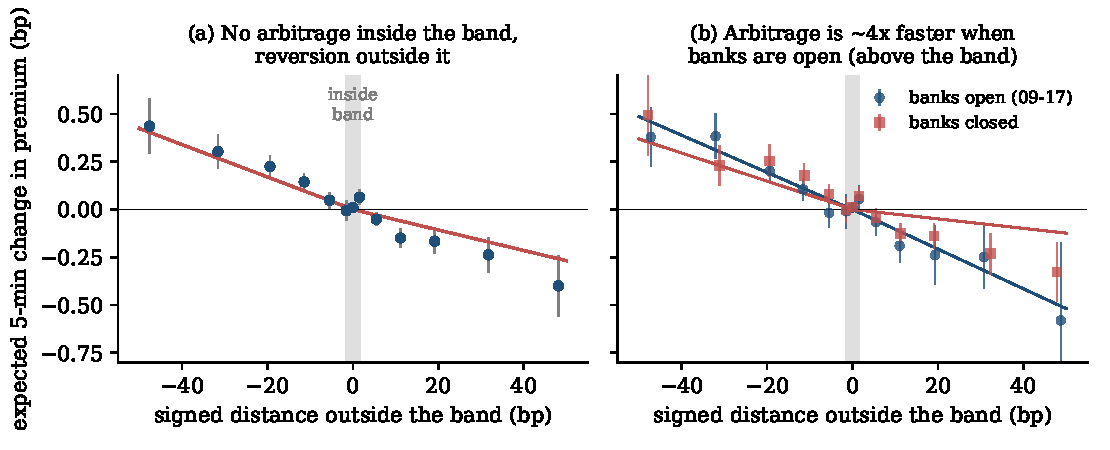
\includegraphics[width=\textwidth]{figures/hero.pdf}
\caption{\textbf{Arbitrage switches on outside a band, and switches on faster when banks are open.} USDT/TRY premium over the interbank rate, five-minute intervals, January 2024 -- August 2026. The horizontal axis is the signed distance of the premium outside its month-specific no-arbitrage band; all observations inside the band are plotted at zero (grey). The vertical axis is the expected change in the premium over the next five minutes, net of order flow and month fixed effects, with 95\% confidence intervals clustered by day. Lines are the fitted threshold model (Table~\ref{tab:emp_main}). Panel (a): full sample. Panel (b): Istanbul business hours versus other hours.}
\label{fig:hero}
\end{figure}

\paragraph{Contribution.}
The paper makes three contributions. It derives the threshold dynamics of a local stablecoin premium from an arbitrageur's problem and obtains closed-form links between capacity, order-flow price impact, the distribution of the premium and the transmission of local information. It turns these links into an estimator that recovers the band, the speed of arbitrage and the long-run impact of order flow from high-frequency data. And it shows, in one of the largest local-currency stablecoin markets, that the speed of arbitrage moves with the availability of the fiat leg, that order flow decomposes by trade size into the demand and arbitrage flows of the model, that a directional transfer rule moved capacity on the constrained side of the band, and that the dollar's price is set in the interbank market.

\paragraph{Related literature.}
The paper sits at the intersection of four literatures.

\emph{Cross-market crypto arbitrage.} \citet{makarov2020trading} document large and persistent cross-country deviations in cryptocurrency prices, link them to capital controls, and show that signed volume co-moves with spreads. \citet{hautsch2024building} show that settlement latency limits cross-exchange arbitrage, and \citet{griffin2020untethered} study the interaction of stablecoin issuance and crypto prices. \citet{hu2023competition} model how arbitrageurs endogenously connect exchanges and show that star-shaped arbitrage networks can arise in equilibrium. Relative to this literature, the paper provides a microstructure model in which a single state variable, arbitrage capacity, governs both the mapping from order flow to the premium and the transmission of local information to the global price, and measures that state variable at minute frequency.

\emph{Stablecoin stability and arbitrage.} \citet{lyons2023stablecoins} study the arbitrage that keeps stablecoins close to their peg. \citet{ma2025stablecoin} show that concentrating primary-market arbitrage in a few authorized intermediaries trades off price stability in normal times against run risk. The network result in Appendix~\ref{app:theory} is the secondary-market, cross-venue analogue of their trade-off. \citet{aldasoro2026stablecoin} show that stablecoin inflows spill over into FX markets and widen parity deviations, and their model features constrained intermediaries whose capital is depleted by losses. Their evidence is a daily panel of cross-country spillovers. This paper identifies the arbitrage technology itself at minute frequency: the inaction band, the speed of adjustment, the transmission of order flow, and the banking-rail state that governs convergence.
% TODO (verify on SSRN before enabling): Shao and Rajapaksa (2026), "The Microstructure of Stablecoin Price Alignment",
% 10-second order books, USDT/USDC route dislocations and finite-depth capacity; distinguish: local-currency premium,
% banking-rail state, threshold capacity. Baulkaran, Jain and Sobanski (2026), "Market Microstructure of Stablecoins:
% Evidence from USDT", 9 exchanges, intraday market quality linked to traditional market hours; distinguish: our
% banking-hours effect is on the speed of arbitrage across the fiat leg, holding order-flow impact fixed.

\emph{Limits to arbitrage and slow-moving capital.} The arbitrageur problem builds on \citet{shleifer1997limits}, \citet{gromb2002equilibrium}, \citet{brunnermeier2009market}, \citet{mitchell2007slow} and \citet{duffie2010presidential}. Deviations from covered interest parity \citep{du2018deviations} are a leading example in traditional markets of arbitrage-capacity-driven basis. The band structure echoes the commodity-points literature in international economics \citep{dumas1992dynamic, obstfeld1997nonlinear} and threshold cointegration \citep{balke1997threshold, hansen2002testing}. Here the threshold is derived from an arbitrageur's optimization and connected to order flow and price discovery.

\emph{Fragmentation and price discovery.} The price-discovery result complements the information-share approach of \citet{hasbrouck1995one} and \citet{gonzalo1995estimation}, which is built on linear error correction. Under threshold arbitrage, the contribution of a venue to price discovery depends on the size of the information it receives, so linear information shares average over economically distinct regimes. \citet{lehar2024fragmentation} show how fixed costs fragment liquidity across fee tiers within a decentralized exchange. This paper studies fragmentation across currencies and its implications for convergence.


The remainder of the paper is organized as follows. Section~\ref{sec:model} presents the model and Section~\ref{sec:implications} its predictions. Section~\ref{sec:empirics} describes the data and the empirical strategy, and Section~\ref{sec:evidence} presents the evidence. Section~\ref{sec:conclusion} concludes. Appendix~\ref{app:proofs} contains proofs, Appendix~\ref{app:theory} further theoretical results, and Appendix~\ref{sec:mc} Monte Carlo evidence on the estimator.

%=====================================================================
\section{Model}\label{sec:model}
%=====================================================================

\subsection{Markets and the premium}

There are two markets for the same dollar stablecoin. In the \emph{local} market the stablecoin trades against a local currency; in the \emph{global} market it trades against the U.S. dollar (or a dollar benchmark such as a deep USDT/USD or USDC/USDT book). Let $P^L_t$ denote the local price converted into dollars at a reference exchange rate, and $P^G_t$ the global dollar price. The object of interest is the log premium
\[
b_t \equiv \log P^L_t - \log P^G_t .
\]
In a frictionless integrated market $b_t\equiv 0$. Which exchange rate is used for the conversion determines the economic interpretation. Converting at the official rate makes $b_t$ a measure of the parallel-market premium, while converting at a contemporaneous local market rate (for example, a local BTC/USDT cross) isolates the stablecoin-specific basis. The model applies to either.

Time is continuous. Three forces move the premium.

\emph{Non-arbitrage order flow.} End users (households seeking dollar exposure, importers, remitters) generate signed order flow $q_t$ in the local market, measured as buyer-initiated minus seller-initiated volume. Absent arbitrage, order flow moves the premium with primitive impact $\beta>0$.

\emph{Arbitrage flow.} A competitive arbitrage sector chooses a flow $a_t$ (units per unit time). A positive $a_t$ sells the stablecoin locally and buys it globally, which lowers the premium. Arbitrage moves the local price with impact $\lambda_L$ and the global price with impact $\lambda_G$, so its effect on the premium is $\lambda\equiv\lambda_L+\lambda_G$.

\emph{Noise.} Everything else, including transient liquidity shocks and quote noise, is captured by $\sigma\,dW_t$, where $W$ is a standard Brownian motion.

\subsection{The arbitrage sector}

\begin{assumption}[Arbitrage technology]\label{ass:arb}
Arbitrage in the positive (negative) direction incurs a proportional cost $c^+>0$ ($c^->0$) per unit, reflecting fees, on/off-ramp costs, FX access and transfer frictions. Holding a flow of size $|a|$ incurs a convex balance-sheet and inventory cost $a^2/(2K^\pm)$, where $K^\pm>0$ is the \emph{arbitrage capacity} in each direction. The arbitrage sector chooses $a_t$ to maximize flow profit
\begin{equation}\label{eq:arbprofit}
\Pi(a;b) =
\begin{cases}
ab - c^+a - \dfrac{a^2}{2K^+}, & a\ge 0,\\[8pt]
ab + c^-a - \dfrac{a^2}{2K^-}, & a<0.
\end{cases}
\end{equation}
\end{assumption}

The proportional cost $c^\pm$ captures every friction that scales with the size of the trade: exchange and network fees, the spread paid on the fiat leg, and the expected cost of on- and off-ramps. Capacity $K^\pm$ captures everything that makes the \emph{marginal} unit costlier: finite capital, inventory risk while transfers settle, counterparty limits at banks and payment providers, and withdrawal limits at exchanges. Allowing both to depend on direction is essential in capital-controlled economies. Buying stablecoins with local currency and moving the dollars abroad is generally harder than the reverse, so one expects $c^+\neq c^-$ and $K^+\neq K^-$.

\begin{proposition}[Optimal arbitrage]\label{prop:policy}
Under Assumption~\ref{ass:arb}, the unique optimal arbitrage flow is
\begin{equation}\label{eq:policy}
a^*(b) = K^+\pos{b-c^+} - K^-\pos{-b-c^-}.
\end{equation}
In particular, $a^*(b)=0$ for $b\in[-c^-,c^+]$; outside this \emph{no-arbitrage band}, arbitrage flow is linear in the excess premium with slope equal to capacity. In the symmetric case, $a^*(b)=K\,\sgn(b)\pos{|b|-c}$.
\end{proposition}

The policy is the soft-thresholding operator familiar from statistics. Its two parameters play distinct economic roles. The friction $c$ determines \emph{whether} arbitrage is active; capacity $K$ determines \emph{how strongly} it responds once active. Figure~\ref{fig:policy}(a) plots the policy.

\begin{remark}[Static versus dynamic arbitrage]
Proposition~\ref{prop:policy} treats arbitrage as a flow decision. In a fully dynamic model with fixed costs, the option value of waiting widens the band beyond the static cost, as in \citet{dumas1992dynamic}. The structure of the solution (inaction inside a band, active trading outside it) is preserved. The band $c^\pm$ estimated in Section~\ref{sec:empirics} should therefore be read as an \emph{effective} threshold that includes any such option value. More generally, for any convex cost $C(a)$ with $C'(0^+)=c^+$ and $C'(0^-)=-c^-$, the optimal policy is $a^*(b)=(C')^{-1}(b)$ outside $[-c^-,c^+]$ and zero inside, so all qualitative results below survive. Only the closed forms rely on the quadratic specification.
\end{remark}

\begin{remark}[Settlement latency and the location of the band]\label{rem:carry}
Cross-border stablecoin arbitrage is not instantaneous. Fiat legs settle with a delay, exchanges can hold withdrawals, and transfers may be subject to compliance reviews. Suppose a round trip ties up capital for a period $\tau$, during which the arbitrageur holds dollar-denominated inventory rather than local-currency deposits. The arbitrageur then forgoes the interest differential $(i-i^*)$ over $\tau$ in \emph{both} directions, so the band becomes $[-c^- - (i-i^*)\tau,\; c^+ + (i-i^*)\tau]$. In a high-interest-rate economy this term is large. At a 45\% annual lira rate, a 48-hour withdrawal hold adds roughly $25$ bp to each edge of the band. Directional frictions, such as limits on outbound stablecoin transfers, raise only one edge. They therefore shift the band's location and, by Proposition~\ref{prop:stationary}(b), the average premium. Empirically, we estimate the edges $\ell\equiv-c^-$ and $u\equiv c^+$ freely, so the band need not contain zero.
\end{remark}

\subsection{Premium dynamics}

Combining non-arbitrage order flow, optimal arbitrage and noise, the premium satisfies
\begin{equation}\label{eq:sde}
db_t = \Big(\beta q_t - \lambda\big[K^+\pos{b_t-c^+} - K^-\pos{-b_t-c^-}\big]\Big)dt + \sigma\,dW_t .
\end{equation}
We write $\kappa^\pm\equiv\lambda K^\pm$ and call it \emph{effective arbitrage capacity}: the speed at which arbitrage closes a dislocation, which combines the balance-sheet capacity $K^\pm$ of the arbitrage sector with the price impact $\lambda$ of its trades. Effective capacity is the object the data identify. Within a market, $\lambda$ reflects the depth of the two legs, so variation in $\kappa$ across adjacent states with the same order-flow impact $\beta$ is variation in $K$. We write
\[
\mu(b) \equiv -\kappa^+\pos{b-c^+} + \kappa^-\pos{-b-c^-}
\]
for the arbitrage component of the drift; Equation~\eqref{eq:sde} is a threshold diffusion. Its drift is identically zero on the band, linear outside it, and kinked at $-c^-$ and $c^+$. Since $\mu$ is Lipschitz, \eqref{eq:sde} has a unique strong solution for any adapted, locally integrable order-flow process $q$.

%=====================================================================
\section{Predictions}\label{sec:implications}
%=====================================================================

\subsection{Inaction and state-dependent reversion}

\begin{proposition}[State-dependent reversion]\label{prop:reversion}
Let $q\equiv 0$.
\begin{enumerate}[label=(\alph*)]
\item \emph{Inaction.} For $b_0\in(-c^-,c^+)$, let $\tau$ be the first exit time from the band. The stopped premium $b_{t\wedge\tau}$ is a martingale, and
\[
\E[\tau\mid b_0] = \frac{(c^+-b_0)(b_0+c^-)}{\sigma^2}.
\]
\item \emph{Exponential correction outside the band.} If $\sigma=0$ and $b_0>c^+$, then $b_t = c^+ + (b_0-c^+)e^{-\kappa^+ t}$. The excess premium has half-life
\[
t_{1/2}^+ = \frac{\ln 2}{\lambda K^+},
\]
and symmetrically $t_{1/2}^-=\ln 2/(\lambda K^-)$ for $b_0<-c^-$.
\item \emph{Large dislocations revert faster.} The proportional reversion speed $\rho(b)\equiv-\mu(b)/b$ equals zero on the band and $\kappa^+(1-c^+/b)$ for $b>c^+$ (symmetrically for $b<-c^-$). It is non-decreasing in $|b|$ and converges to $\kappa^\pm$ as $|b|\to\infty$.
\end{enumerate}
\end{proposition}

Proposition~\ref{prop:reversion} contains the first set of testable predictions. Small premia do not mean-revert; they wander until they hit the edge of the band, with an expected waiting time that rises with the square of the band width. Large premia revert, and do so proportionally faster the larger they are. A linear error-correction model imposes a constant $\rho$. Figure~\ref{fig:policy}(b) shows that any constant necessarily overstates reversion for small dislocations and understates it for large ones. The half-life formula gives capacity a direct, observable counterpart: halving capacity doubles the half-life of a dislocation.

\begin{figure}[t]
\centering
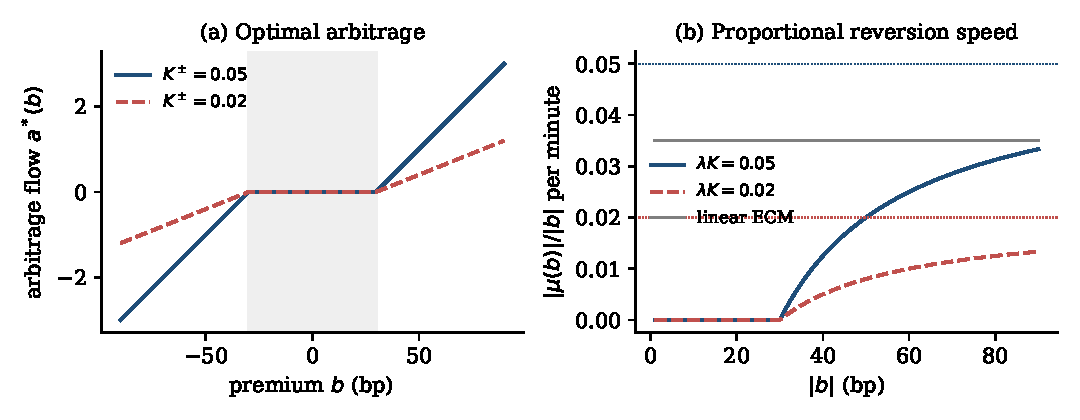
\includegraphics[width=\textwidth]{figures/fig1_policy.pdf}
\caption{\textbf{Optimal arbitrage and state-dependent reversion.} Panel (a) plots the optimal arbitrage flow $a^*(b)$ of Proposition~\ref{prop:policy} for two levels of capacity with $c^\pm=30$ bp; the shaded region is the no-arbitrage band. Panel (b) plots the proportional reversion speed $|\mu(b)|/|b|$ of Proposition~\ref{prop:reversion}(c), with $\lambda=1$; dotted lines mark the asymptotes $\kappa=\lambda K$. The flat grey line is a constant-speed linear error-correction model.}
\label{fig:policy}
\end{figure}

\subsection{Order flow, price impact and volume}

\begin{proposition}[Long-run price impact]\label{prop:impact}
Let $\sigma=0$ and $q_t\equiv q$ constant.
\begin{enumerate}[label=(\alph*)]
\item If $q>0$, then from any initial condition $b_t\to b^*$, where
\[
b^* = c^+ + \frac{\beta q}{\lambda K^+}.
\]
If $q<0$, $b_t\to -c^- + \beta q/(\lambda K^-)$. If $q=0$, $b_t$ converges to the closest point of the band.
\item The long-run price impact of order flow is
\[
\frac{\partial b^*}{\partial q} = \frac{\beta}{\lambda K^\pm},
\]
which is decreasing in capacity.
\item In the steady state, arbitrage flow equals $a^* = \beta q/\lambda$, which does not depend on $(c^\pm,K^\pm)$. Total local volume, $|q|+|a^*|$, is therefore independent of arbitrage capacity, while the premium is decreasing in it.
\end{enumerate}
\end{proposition}

Part (c) is the paper's central observational-equivalence result. In steady state arbitrageurs must absorb the full non-arbitrage flow, scaled by relative impact, whatever their capacity. Capacity determines only the premium at which they are willing to do so. Volume reveals demand; the premium reveals capacity.

\begin{corollary}[Volume, premia and demand across markets]\label{cor:equivalence}
Consider two local markets $i\in\{A,B\}$ with parameters $(\beta_i,\lambda_i,c_i,K_i)$ and persistent order flow $q_i>0$. Then
\[
b^*_A - c_A = b^*_B - c_B
\quad\Longleftrightarrow\quad
\frac{\beta_A q_A}{\lambda_A K_A} = \frac{\beta_B q_B}{\lambda_B K_B}.
\]
In particular, equal excess premia are consistent with arbitrarily different demand, provided capacity differs in proportion. Conversely, equal demand and impact ($\beta_Aq_A=\beta_Bq_B$, $\lambda_A=\lambda_B$) produce excess premia in inverse proportion to capacity.
\end{corollary}

Corollary~\ref{cor:equivalence} explains why comparisons of premia across countries, or across episodes within a country, cannot by themselves be read as comparisons of demand. Separating demand from capacity requires the joint dynamics of the premium and order flow, which is exactly what the estimator of Section~\ref{sec:empirics} uses.

\subsection{Capacity depletion and the arbitrage throughput limit}

Capacity is depletable. Arbitrage ties up capital in transit, exhausts withdrawal limits and banking lines, and accumulates inventory that must be unwound. We now let capacity respond to arbitrage activity. Focus on the region $b>c^+$ and drop direction superscripts:
\begin{equation}\label{eq:Kdyn}
dK_t = \big[\xi(\bar K - K_t) - \chi\,|a^*_t|\big]dt, \qquad a^*_t = K_t\pos{b_t-c},
\end{equation}
where $\bar K$ is normal-times capacity, $\xi$ is the rate at which capacity replenishes (capital is redeployed, limits reset), and $\chi$ is the rate at which arbitrage activity consumes it.

\begin{proposition}[Throughput limit and convex impact]\label{prop:depletion}
Let $\sigma=0$, $q_t\equiv q>0$, and let $(b_t,K_t)$ follow~\eqref{eq:sde} and~\eqref{eq:Kdyn} with $K_0>0$. Define the \emph{arbitrage throughput limit} $\bar a\equiv\xi\bar K/\chi$ and the critical order flow
\[
q_{crit} \equiv \frac{\lambda\bar a}{\beta} = \frac{\xi\lambda\bar K}{\chi\beta}.
\]
\begin{enumerate}[label=(\alph*)]
\item If $q<q_{crit}$, there is a unique steady state,
\[
K^* = \bar K\Big(1-\frac{q}{q_{crit}}\Big),\qquad
b^* = c + \frac{\beta q}{\lambda\bar K\,(1-q/q_{crit})},
\]
and it is locally asymptotically stable. The long-run price impact
\[
\frac{\partial b^*}{\partial q} = \frac{\beta}{\lambda\bar K\,(1-q/q_{crit})^2}
\]
is increasing and convex in $q$ and diverges as $q\uparrow q_{crit}$.
\item If $q>q_{crit}$, no steady state exists, and for any initial condition
\[
\liminf_{t\to\infty}\frac{b_t}{t} \;\ge\; \beta\,(q-q_{crit}) > 0 .
\]
\end{enumerate}
\end{proposition}

Proposition~\ref{prop:depletion} identifies the binding constraint in stressed markets. The binding constraint is the flow $\bar a=\xi\bar K/\chi$, the rate at which the arbitrage sector can sustainably process trades. Demand above this throughput limit cannot be absorbed at any premium, and the premium drifts away. This is the mechanism behind sudden de-pegs of local stablecoin prices during currency crises and capital-control tightening. Demand surges, arbitrage turns on, capacity is consumed, and future corrections slow down, which lets the premium keep widening. Figure~\ref{fig:capacity} in Appendix~\ref{app:theory} illustrates both regimes. In the illustrative calibration, depletion doubles the peak premium and raises the half-life of the subsequent correction from 14 minutes to more than six hours.

\begin{remark}[A settlement queue]\label{rem:queue}
Let $I_t\equiv\bar K-K_t$ be the balance-sheet capacity tied up in trades that have been executed but not yet settled. Equation~\eqref{eq:Kdyn} becomes
\[
\dot I_t=\chi\,|a_t|-\xi I_t ,
\]
a fluid queue in which arbitrage trades arrive at rate $\chi|a_t|$ and settlement jobs, such as bank transfers and exchange withdrawals, are completed at rate $\xi$ per unit in process. In steady state the work in process is $I^*=\chi a/\xi$, and it cannot exceed total capacity $\bar K$, so throughput is bounded by $\bar a=\xi\bar K/\chi$. Market clearing, $\lambda a=\beta q$, then gives $q_{crit}=\lambda\xi\bar K/(\chi\beta)$. The throughput limit of Proposition~\ref{prop:depletion} is the capacity of the settlement queue, and the divergence of price impact as $q\uparrow q_{crit}$ is its heavy-traffic limit: as utilization $q/q_{crit}$ approaches one, free capacity $K^*=\bar K(1-q/q_{crit})$ vanishes and the premium needed to clear the market explodes. Settlement speed $\xi$, which depends on banking hours and withdrawal holds, enters the limit one-for-one.
\end{remark}


\subsection{Price discovery: who discovers the dollar?}

We now ask how information that arrives first in the local market is transmitted to the global price. Let the local price jump by $\delta>0$ at $t=0$ because informed local order flow reveals news about the common dollar value (for example, news about the issuer, or about the dollar's local purchasing power that global participants learn only through prices). Before the shock $b_{0^-}=0$. Arbitrage moves the local price by $-\lambda_L a\,dt$ and the global price by $+\lambda_G a\,dt$. Define the global leg's share of arbitrage impact $\omega\equiv\lambda_G/(\lambda_L+\lambda_G)$.

\begin{proposition}[Local information transmission]\label{prop:discovery}
Let $\sigma=0$ and $q_t\equiv0$ for $t>0$. The global price at horizon $h$ satisfies
\[
S_h(\delta)\;\equiv\;\frac{\log P^G_h-\log P^G_0}{\delta} = \omega\Big(1-\frac{c^+}{\delta}\Big)_+\big(1-e^{-\lambda K^+ h}\big).
\]
Consequently:
\begin{enumerate}[label=(\alph*)]
\item local information shocks smaller than the band ($\delta\le c^+$) are never transmitted to the global price;
\item the long-run share $S_\infty(\delta)=\omega(1-c^+/\delta)_+$ is decreasing in the friction and independent of capacity;
\item at any finite horizon, $S_h(\delta)$ is increasing in capacity, and the half-life of transmission is $\ln2/(\lambda K^+)$.
\end{enumerate}
\end{proposition}

Frictions determine how much local information ever reaches the global price; capacity determines how fast it gets there (Figure~\ref{fig:discovery} in Appendix~\ref{app:theory}). A market with heavy trading but a wide band, or one whose arbitrage capacity is impaired, can be very active and still contribute almost nothing to the price of the dollar elsewhere. This is consistent with the finding of \citet{makarov2020trading} that more segmented, higher-premium venues contribute less to global price discovery, and it explains that finding through $(c,K)$. A further implication concerns measurement. Linear information-share measures \citep{hasbrouck1995one, gonzalo1995estimation} average $S_h(\delta)$ over the distribution of shock sizes. They therefore depend on the volatility regime and can change sharply with no change in market structure.


%=====================================================================
\section{Data and empirical strategy}\label{sec:empirics}
%=====================================================================

Turkey is a natural laboratory for the model. Domestic demand for dollar assets is strong and persistent, the lira experienced a large political shock during the sample, policy rates were high enough to make the carry cost of settlement latency in Remark~\ref{rem:carry} economically large, and access to the fiat leg of the arbitrage runs through domestic banking rails whose availability varies over the day.

\paragraph{Local market.} One-minute USDT/TRY candles come from Binance's public data archive, from 2 January 2024 to 31 August 2026. For each minute the archive reports volume, the number of trades, quote volume and \emph{taker-buy} volume. The local price $P^L_t$ is the minute volume-weighted average price (quote volume divided by volume). Signed order flow is taker-buy minus taker-sell volume, $\mathit{OFI}_t=2\,\mathit{TBV}_t-V_t$, in USDT. The market is deep: the median minute has 90 trades and 36 thousand USDT of volume (Table~\ref{tab:summary}).

\paragraph{Benchmark.} The dollar price is the interbank USD/TRY mid-quote from Dukascopy one-minute candles, whose median relative bid-ask spread is about 1 bp. The sample uses minutes with interbank activity on weekdays, excludes the 20:30--22:30 UTC rollover window, and discards minutes with $|b_t|>10\%$. The premium is $b_t=10^4(\log P^L_t-\log P^G_t)$ in basis points.

\paragraph{Where the friction sits.} On the same exchange, the USDT/TRY price and the USDT price implied by the BTC/TRY and BTC/USDT order books differ with a standard deviation of $2.4$ bp; this triangular arbitrage moves no fiat money. The premium over the interbank rate has a standard deviation of $56$ bp. The relevant frictions are those of the fiat and cross-border leg, which is what $c$ and $K$ measure.

\begin{table}[t]
\centering
\caption{\textbf{Summary statistics: USDT/TRY, January 2024 -- August 2026}}
\label{tab:summary}
\footnotesize
\resizebox{\ifdim\width>\textwidth\textwidth\else\width\fi}{!}{\begin{tabular}{lrrrrrr}
\toprule
 & Mean & SD & P1 & P50 & P99 & $N$ \\
\midrule
Premium $b_t$ (bp), 1-min & 18.43 & 56.43 & -60.06 & 5.76 & 269.96 & 808,473 \\
Premium (bp), 5-min average & 18.30 & 56.34 & -60.22 & 5.62 & 269.74 & 162,624 \\
USDT/TRY volume (thousand USDT per min) & 64.91 & 129.97 & 1.13 & 36.42 & 543.61 & 808,473 \\
Signed order flow (thousand USDT per min) & 9.12 & 112.69 & -212.43 & 2.46 & 210.12 & 808,473 \\
Trades per minute & 143.40 & 204.96 & 8.00 & 90.00 & 952.00 & 808,473 \\
Interbank USD/TRY bid-ask spread (bp) & 1.26 & 1.09 & 0.50 & 0.97 & 6.74 & 15,149 \\
Triangular basis USDT/TRY vs.\ BTC cross (bp) & -0.13 & 2.38 & -6.18 & -0.10 & 5.68 & 1,378,099 \\
\bottomrule
\end{tabular}
}
\begin{minipage}{0.95\textwidth}
\footnotesize\vspace{4pt}
\emph{Notes:} One-minute data on weekdays, excluding 20:30--22:30 UTC. The premium is the log difference between the Binance USDT/TRY minute VWAP and the Dukascopy interbank USD/TRY mid. Signed order flow is taker-buy minus taker-sell volume. The triangular basis compares USDT/TRY with the cross rate implied by BTC/TRY and BTC/USDT on the same exchange (all days).
\end{minipage}
\end{table}

\paragraph{Estimating equation.} The premium is averaged over non-overlapping five-minute intervals, which removes most of the bid-ask bounce in the local price, and order flow is summed over the same interval and standardized by its within-month standard deviation. An Euler discretization of~\eqref{eq:sde} gives
\begin{equation}\label{eq:emp}
\Delta b_t=\alpha_m+\beta\,\mathit{OFI}_t-\kappa^+\pos{b_{t-1}-u_m}+\kappa^-\pos{\ell_m-b_{t-1}}+\varepsilon_t,
\end{equation}
where $t$ indexes five-minute intervals, $\alpha_m$ is a month fixed effect, $[\ell_m,u_m]$ is the month's no-arbitrage band, and $\kappa^\pm=\lambda K^\pm\Delta$ is effective capacity per interval. The structural objects are the band, the speeds $\kappa^\pm$, the primitive impact $\beta$ (in bp per one-standard-deviation five-minute order-flow shock) and the long-run impact $\beta/\kappa^\pm$ of Proposition~\ref{prop:impact}. Since $K$ and $\lambda$ enter as a product, comparisons of $\kappa$ across states of the same market with the same order-flow impact $\beta$ are comparisons of balance-sheet capacity.

\paragraph{Month-specific bands.} The level of the premium moves at low frequency (Figure~\ref{fig:emp_premium}): it averaged more than 100 bp in the first half of 2024, fluctuated around zero in 2025, and turned into a discount of 10--25 bp in 2026. Remark~\ref{rem:carry} attributes such movements to carry and directional frictions, which shift the band. The edges $(\ell_m,u_m)$ are therefore profiled month by month over a 1 bp grid, subject to $\ell_m\le u_m$ and 5\% trimming. Given the bands, the slopes of~\eqref{eq:emp} are estimated by pooled OLS. Thresholds are super-consistent \citep{hansen2000sample}, so slope inference treats them as known. Standard errors are clustered by day. Linearity is tested against the threshold model with the sup-LR statistic \citep{hansen1996inference, hansen2002testing}, summed across months, with a day-clustered wild bootstrap under the linear null. Appendix~\ref{sec:mc} shows that the profiled estimator recovers the band, the speeds and the order-flow impact at sample sizes of two weeks of minute data.

\begin{figure}[t]
\centering
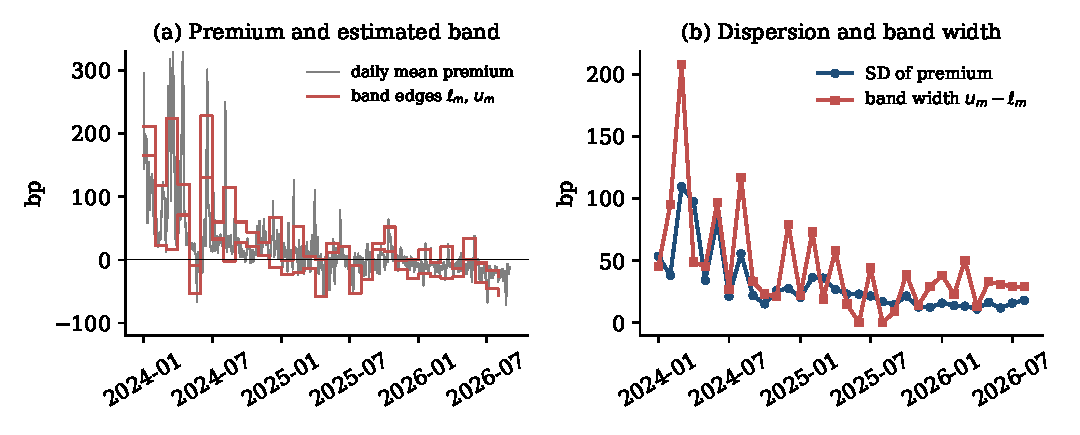
\includegraphics[width=\textwidth]{figures/emp_premium.pdf}
\caption{\textbf{The USDT/TRY premium over the interbank rate.} Panel (a): daily mean premium and the estimated monthly band edges $\ell_m$ and $u_m$. Panel (b): monthly standard deviation of the five-minute premium and the width of the estimated band.}
\label{fig:emp_premium}
\end{figure}

%=====================================================================
\section{Evidence}\label{sec:evidence}
%=====================================================================

\subsection{Threshold dynamics}

Table~\ref{tab:emp_main} reports the main estimates. Column (1) is a linear error-correction model with month fixed effects; it attributes slow, uniform reversion to the premium ($\hat\kappa=0.0039$ per five minutes). Column (2) estimates the threshold model. Outside the band the premium reverts at $\hat\kappa^+=0.0054$ above it and $\hat\kappa^-=0.0085$ below it, both significant at 1\%. Column (3) adds a linear reversion term that is active only inside the band; its coefficient is $-0.0006$ with a standard error of $0.0007$. Inside the band the premium is a martingale, as Proposition~\ref{prop:reversion}(a) predicts. The median band is 32 bp wide and contains 39\% of the intervals. Summed across months, the sup-LR statistic is 464, and the wild bootstrap rejects linear error correction with a $p$-value of $0.01$, the smallest attainable with 99 draws.

\begin{table}[t]
\centering
\caption{\textbf{Threshold arbitrage in the USDT/TRY premium}}
\label{tab:emp_main}
\footnotesize
\resizebox{\ifdim\width>\textwidth\textwidth\else\width\fi}{!}{\begin{tabular}{lcccc}
\toprule
 & (1) & (2) & (3) & (4) \\
\midrule
OFI$_t$ & $0.603^{***}$ & $0.604^{***}$ & $0.604^{***}$ & $0.635^{***}$ \\
 & $(0.030)$ & $(0.030)$ & $(0.030)$ & $(0.032)$ \\
$-(b_{t-1}-u_m)_+$ \;[$\kappa^+$] &  & $0.0054^{***}$ & $0.0054^{***}$ & $0.0025^{*}$ \\
 &  & $(0.0013)$ & $(0.0013)$ & $(0.0013)$ \\
$(\ell_m-b_{t-1})_+$ \;[$\kappa^-$] &  & $0.0085^{***}$ & $0.0085^{***}$ & $0.0074^{***}$ \\
 &  & $(0.0025)$ & $(0.0025)$ & $(0.0018)$ \\
$-b_{t-1}$ \;[linear $\kappa$] & $0.0039^{***}$ &  &  &  \\
 & $(0.0006)$ &  &  &  \\
$-(b_{t-1}-m_m)\cdot\mathbb 1\{\text{in band}\}$ &  &  & $-0.0006$ &  \\
 &  &  & $(0.0007)$ &  \\
OFI$_t\times$BH &  &  &  & $-0.052$ \\
 &  &  &  & $(0.033)$ \\
$-(b_{t-1}-u_m)_+\times$BH &  &  &  & $0.0079^{***}$ \\
 &  &  &  & $(0.0014)$ \\
$(\ell_m-b_{t-1})_+\times$BH &  &  &  & $0.0023$ \\
 &  &  &  & $(0.0018)$ \\
\midrule
Month fixed effects & Yes & Yes & Yes & Yes \\
Month-specific band $[\ell_m,u_m]$ & No & Yes & Yes & Yes \\
$N$ & 162,624 & 162,624 & 162,624 & 162,624 \\
Within $R^2$ & 0.042 & 0.042 & 0.042 & 0.043 \\
\bottomrule
\end{tabular}
}
\begin{minipage}{0.95\textwidth}
\footnotesize\vspace{4pt}
\emph{Notes:} Dependent variable: five-minute change in the premium (bp). OFI is standardized within month. $[\ell_m,u_m]$ is the band estimated month by month; $m_m$ is its midpoint. BH is an indicator for Istanbul business hours (09:00--17:00). Standard errors clustered by day in parentheses. ***, **, * denote significance at 1\%, 5\%, 10\%.
\end{minipage}
\end{table}

Table~\ref{tab:emp_bins} and Figure~\ref{fig:emp_drift} trace reversion by the size of the dislocation. Inside the band, proportional reversion is zero. Beyond 10 bp outside the band, reversion switches on at 0.5--0.6\% per five minutes. Within the first 5 bp outside the band the premium continues to drift outward, and between 5 and 10 bp it is flat; this is the transition toward the steady state $b^*=c+\beta q/(\lambda K)$ that Proposition~\ref{prop:impact} predicts under persistent order flow. The largest dislocations, concentrated in the first half of 2024, revert at 0.37\% per five minutes, in line with the capacity depletion of Proposition~\ref{prop:depletion}.

\begin{figure}[t]
\centering
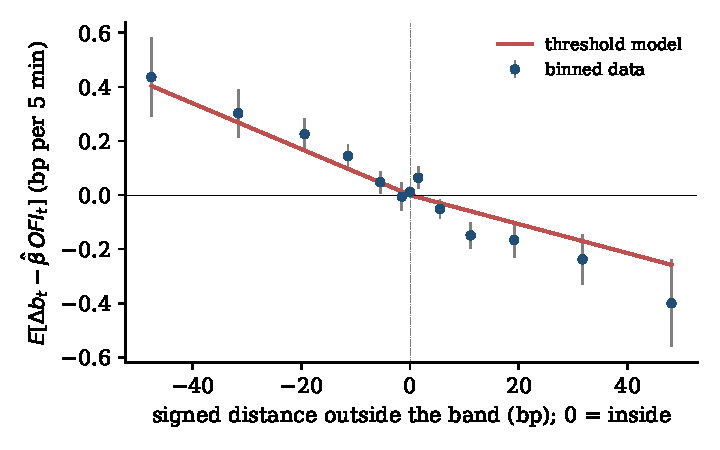
\includegraphics[width=0.66\textwidth]{figures/emp_drift.pdf}
\caption{\textbf{Expected premium change by position relative to the band.} Mean five-minute change in the premium net of the order-flow component, by signed distance outside the month-specific band (0 = inside the band), net of month fixed effects, with 95\% confidence intervals clustered by day. Dislocations more than 60 bp outside the band are omitted for readability. The red line is the fitted drift of column (2) of Table~\ref{tab:emp_main}.}
\label{fig:emp_drift}
\end{figure}

\begin{table}[t]
\centering
\caption{\textbf{Reversion by size of dislocation}}
\label{tab:emp_bins}
\footnotesize
\resizebox{\ifdim\width>\textwidth\textwidth\else\width\fi}{!}{\begin{tabular}{lcccc}
\toprule
 & Mean distance (bp) & Reversion per 5 min, $\hat\rho$ & Half-life (min) & $N$ \\
\midrule
Inside band, inner half & 6.9 & $-0.0028$ $(0.0020)$ & $\infty$ & 32,221 \\
Inside band, outer half & 21.6 & $-0.0020$ $(0.0006)$ & $\infty$ & 31,020 \\
Outside, excess $\in(0,5]$ bp & 2.5 & $-0.0154$ $(0.0055)$ & $\infty$ & 20,099 \\
Outside, excess $\in(5,10]$ bp & 7.4 & $0.0004$ $(0.0023)$ & 7868 & 18,562 \\
Outside, excess $\in(10,20]$ bp & 14.5 & $0.0052$ $(0.0011)$ & 662 & 24,682 \\
Outside, excess $\in(20,40]$ bp & 28.4 & $0.0058$ $(0.0008)$ & 593 & 19,918 \\
Outside, excess $>40$ bp & 81.9 & $0.0037$ $(0.0006)$ & 949 & 16,122 \\
\bottomrule
\end{tabular}
}
\begin{minipage}{0.95\textwidth}
\footnotesize\vspace{4pt}
\emph{Notes:} Proportional reversion $\hat\rho$ is the sum of reversion toward the band (net of $\hat\beta\,\mathit{OFI}_t$) divided by the sum of distances, measured from the band midpoint inside the band and from the nearest edge outside it. Delta-method standard errors clustered by day. Half-lives in minutes.
\end{minipage}
\end{table}

\subsection{Capacity follows the banking day}

During Istanbul business hours, banks process transfers and the fiat leg of the arbitrage can be executed; outside them, the stablecoin market keeps trading while the fiat leg slows down. Column (4) of Table~\ref{tab:emp_main} interacts the reversion terms and order flow with an indicator for 09:00--17:00 Istanbul time. Above the band, the speed of arbitrage is $0.0025$ outside business hours and $0.0104$ during them; the difference, $0.0079$ (s.e.\ $0.0014$), is a fourfold increase. The primitive impact of order flow is statistically the same in the two states ($0.64$ and $0.58$). By Proposition~\ref{prop:impact}, the long-run impact of a sustained one-standard-deviation order-flow imbalance is $\beta/\kappa^+\approx 56$ bp during business hours and $257$ bp outside them. This is Corollary~\ref{cor:equivalence} inside a single market: the same demand moves the premium nearly five times as much when capacity is low.

Table~\ref{tab:emp_quality} confirms that the interbank benchmark drives none of this. Column (2) keeps only intervals in which the interbank market is actively quoted, defined as tick activity above the 25th percentile of business hours; the business-hours increase in $\kappa^+$ is $0.0088$ (s.e.\ $0.0016$). Columns (3) and (4) split the correction into the two legs. Noisy night-time interbank quotes would show up as night-time reversion in the interbank leg; the interbank leg shows no reversion in either state, and the entire business-hours effect sits in the stablecoin price.

\begin{table}[t]
\centering
\caption{\textbf{Banking hours and the interbank benchmark}}
\label{tab:emp_quality}
\footnotesize
\resizebox{\ifdim\width>\textwidth\textwidth\else\width\fi}{!}{\begin{tabular}{lcccc}
\toprule
 & \multicolumn{2}{c}{$\Delta b_t$} & $\Delta\log P^L_t$ & $\Delta\log P^G_t$ \\
\cmidrule(lr){2-3}\cmidrule(lr){4-4}\cmidrule(lr){5-5}
 & All & Active interbank & All & All \\
 & (1) & (2) & (3) & (4) \\
\midrule
$-(b_{t-1}-u_m)_+$ [$\kappa^+$, banks closed] & $0.0025^{*}$ & $0.0016$ & $0.0024^{*}$ & $-0.0000$ \\
 & $(0.0013)$ & $(0.0017)$ & $(0.0013)$ & $(0.0004)$ \\
$\quad\times$ banks open & $0.0079^{***}$ & $0.0088^{***}$ & $0.0074^{***}$ & $-0.0006$ \\
 & $(0.0014)$ & $(0.0016)$ & $(0.0016)$ & $(0.0004)$ \\
$(\ell_m-b_{t-1})_+$ [$\kappa^-$, banks closed] & $0.0074^{***}$ & $0.0081^{***}$ & $0.0059^{***}$ & $-0.0015$ \\
 & $(0.0018)$ & $(0.0023)$ & $(0.0011)$ & $(0.0015)$ \\
$\quad\times$ banks open & $0.0023$ & $0.0028$ & $0.0008$ & $-0.0016$ \\
 & $(0.0018)$ & $(0.0021)$ & $(0.0007)$ & $(0.0016)$ \\
OFI$_t$ [banks closed] & $0.635^{***}$ & $0.699^{***}$ & $0.645^{***}$ & $0.007$ \\
 & $(0.032)$ & $(0.038)$ & $(0.032)$ & $(0.008)$ \\
$\quad\times$ banks open & $-0.052$ & $-0.058$ & $-0.061^{*}$ & $-0.006$ \\
 & $(0.033)$ & $(0.040)$ & $(0.034)$ & $(0.025)$ \\
\midrule
$N$ & 162,624 & 111,037 & 162,624 & 162,624 \\
\bottomrule
\end{tabular}
}
\begin{minipage}{0.95\textwidth}
\footnotesize\vspace{4pt}
\emph{Notes:} Specification~\eqref{eq:emp} with all coefficients interacted with an indicator for Istanbul business hours. Column (2) keeps intervals whose interbank tick activity exceeds the 25th percentile of business-hours intervals. Columns (3) and (4) use the five-minute change in the log USDT/TRY price and in the log interbank rate (bp) as dependent variables. Month fixed effects and month-specific bands throughout; standard errors clustered by day.
\end{minipage}
\end{table}

\paragraph{Friction or capacity?} Closed banks could also widen the band, since settlement latency enters the band through carry (Remark~\ref{rem:carry}). Column (1) of Table~\ref{tab:emp_state} re-estimates the band separately for open and closed hours within each month, with month-by-state fixed effects. Closed-hour bands are wider, 48 bp against 40 bp on average and 34 bp against 24 bp at the median, consistent with longer settlement. With the friction separated out, effective capacity above the band is about five times higher when banks are open: the increment is $0.0067$ (s.e.\ $0.0023$) on a closed-hours speed of $0.0017$. The banking day moves both objects of the model, and the capacity effect holds on its own.

\paragraph{Order flow and arbitrage trades.} Measured order flow can include arbitrageurs' own trades, whereas $q$ in the model is end-user flow. Inside the band $a^*=0$ (Proposition~\ref{prop:policy}), so in-band order flow is end-user flow by construction. Column (2) of Table~\ref{tab:emp_state} estimates $\beta$ from in-band intervals only, which gives $0.64$ in both states, fixes it, and re-estimates the speeds on the order-flow-adjusted premium change. The estimates of effective capacity are unchanged.

\begin{table}[t]
\centering
\caption{\textbf{Separating the friction from effective capacity}}
\label{tab:emp_state}
\footnotesize
\resizebox{\ifdim\width>\textwidth\textwidth\else\width\fi}{!}{\begin{tabular}{lcc}
\toprule
 & State-specific bands & In-band $\beta$, fixed \\
 & (1) & (2) \\
\midrule
$\kappa^+$, banks closed & $0.0017$ & $0.0017$ \\
 & $(0.0015)$ & $(0.0015)$ \\
$\quad\times$ banks open & $0.0067^{***}$ & $0.0067^{***}$ \\
 & $(0.0023)$ & $(0.0023)$ \\
$\kappa^-$, banks closed & $0.0061^{***}$ & $0.0061^{***}$ \\
 & $(0.0012)$ & $(0.0012)$ \\
$\quad\times$ banks open & $0.0082$ & $0.0082$ \\
 & $(0.0054)$ & $(0.0054)$ \\
$\beta$, banks closed & $0.632^{***}$ & $0.641^{***}$ \\
 & $(0.032)$ & $(0.039)$ \\
$\quad\times$ banks open & $-0.047$ & $-0.004$ \\
 & $(0.035)$ & $(0.053)$ \\
\midrule
Mean band width, banks open (bp) & \multicolumn{2}{c}{39.6} \\
Mean band width, banks closed (bp) & \multicolumn{2}{c}{47.6} \\
Difference, closed $-$ open (bp) & \multicolumn{2}{c}{8.0 (8.7)} \\
$N$ & 162,624 & 162,624 \\
\bottomrule
\end{tabular}
}
\begin{minipage}{0.95\textwidth}
\footnotesize\vspace{4pt}
\emph{Notes:} Column (1): bands $[\ell,u]$ profiled separately for each month and banking state (open: 09:00--17:00 Istanbul), month-by-state fixed effects, all slopes interacted with the banks-open indicator. Column (2): $\beta$ estimated on in-band intervals only and held fixed; the dependent variable is $\Delta b_t-\hat\beta\,\mathit{OFI}_t$. Band widths are averages of the monthly estimates; the standard error of the difference is across months. Standard errors clustered by day.
\end{minipage}
\end{table}

Figure~\ref{fig:emp_intraday} shows the same pattern in levels. The mean absolute deviation of the premium from its daily median is about 7 bp in the early afternoon in Istanbul and 13--15 bp late in the evening, when stablecoin volume is still two thirds of its daytime peak.

\begin{figure}[t]
\centering
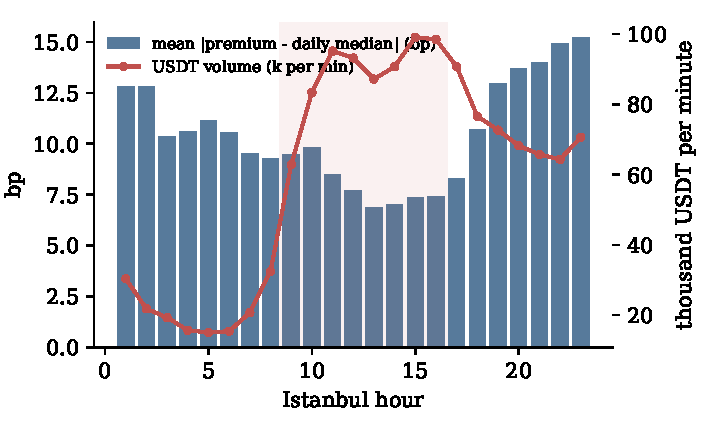
\includegraphics[width=0.66\textwidth]{figures/emp_intraday.pdf}
\caption{\textbf{Intraday pattern.} Bars: mean absolute deviation of the one-minute premium from its daily median, by Istanbul hour (weekdays). Line: mean USDT/TRY volume per minute. The shaded area marks business hours.}
\label{fig:emp_intraday}
\end{figure}

\subsection{Demand and arbitrage in the order flow}

The model has two flows: end-user demand $q$, which pushes the premium, and arbitrage $a^*$, which leans against it once the premium leaves the band. Binance trade-level data allow a direct look at both. Signed order flow is split by the size of each aggressive trade into small ($<$1{,}000 USDT), medium (1{,}000--10{,}000) and large ($\ge$10{,}000) trades, which account for 22\%, 37\% and 41\% of volume, and each class is regressed on the lagged excess premium above and below the month's band (Table~\ref{tab:emp_size}).

Small and medium trades move with the dislocation: they buy when the premium is above the band and sell when it is below it. They are the demand that opens the gap. Large trades move against it: they sell when the premium is above the band and buy when it is below it, the signature of $a^*$ in Proposition~\ref{prop:policy}. Their response follows the banking day. Above the band, large-trade selling is about seven times stronger when banks are open ($-0.30$ against $-0.04$ standard deviations of flow per 100 bp of excess). Large trades also carry the largest price impact ($0.55$ bp per standard deviation, against $0.23$ for medium and zero for small trades). The two flows of the model, and the dependence of the arbitrage flow on the fiat leg, are visible in who trades.

\begin{table}[t]
\centering
\caption{\textbf{Order flow by trade size and the excess premium}}
\label{tab:emp_size}
\footnotesize
\resizebox{\ifdim\width>\textwidth\textwidth\else\width\fi}{!}{\begin{tabular}{lccc}
\toprule
 & \multicolumn{3}{c}{Standardized signed order flow, by trade size} \\
\cmidrule(lr){2-4}
 & Small & Medium & Large \\
 & $<1$k USDT & 1k--10k & $\ge 10$k \\
\midrule
$(b_{t-1}-u_m)_+$ & $0.491^{***}$ & $0.141$ & $-0.042^{*}$ \\
 & $(0.167)$ & $(0.102)$ & $(0.022)$ \\
$\quad\times$ banks open & $0.499^{***}$ & $0.705^{***}$ & $-0.260^{***}$ \\
 & $(0.186)$ & $(0.176)$ & $(0.036)$ \\
$(\ell_m-b_{t-1})_+$ & $-0.800^{***}$ & $-0.693^{***}$ & $0.151^{***}$ \\
 & $(0.100)$ & $(0.094)$ & $(0.025)$ \\
$\quad\times$ banks open & $0.256^{***}$ & $0.408^{***}$ & $-0.086^{***}$ \\
 & $(0.060)$ & $(0.071)$ & $(0.022)$ \\
\midrule
Share of volume & 0.22 & 0.37 & 0.41 \\
Price impact on $\Delta b_t$ (bp per s.d.) & $-0.020$ & $0.225^{***}$ & $0.554^{***}$ \\
 & $(0.061)$ & $(0.019)$ & $(0.032)$ \\
$N$ & \multicolumn{3}{c}{162,624} \\
\bottomrule
\end{tabular}
}
\begin{minipage}{0.95\textwidth}
\footnotesize\vspace{4pt}
\emph{Notes:} Binance USDT/TRY aggregated trades, January 2024 -- August 2026. Signed volume of aggressive trades by size class, summed over five-minute intervals and standardized within month, regressed on the lagged excess premium above and below the month-specific band and its interaction with the banks-open indicator. Coefficients are in standard deviations of flow per 100 bp of excess. The price-impact row regresses $\Delta b_t$ on the three standardized flows and the excess terms. Month fixed effects; standard errors clustered by day.
\end{minipage}
\end{table}

\subsection{Who discovers the dollar?}

Proposition~\ref{prop:discovery} links price discovery to $\omega$, the share of an arbitrage correction borne by the global price. Table~\ref{tab:emp_legs} estimates~\eqref{eq:emp} separately for the local price and the interbank rate. When the premium is above the band, the local price falls at rate $0.0051$ and the interbank rate stays put ($-0.0002$, s.e.\ $0.0004$), so $\hat\omega=0.04$; below the band the interbank coefficient is again insignificant. Stablecoin order flow moves the local price ($0.61$) and leaves the interbank rate unchanged ($0.003$, s.e.\ $0.018$). The dollar's lira price is discovered in the interbank market, and the stablecoin market follows it with a lag set by arbitrage capacity.

\begin{table}[t]
\centering
\caption{\textbf{Which price adjusts?}}
\label{tab:emp_legs}
\footnotesize
\resizebox{\ifdim\width>\textwidth\textwidth\else\width\fi}{!}{\begin{tabular}{lcc}
\toprule
 & $\Delta\log P^L_t$ (USDT/TRY) & $\Delta\log P^G_t$ (USD/TRY) \\
\midrule
OFI$_t$ & $0.609^{***}$ & $0.003$ \\
 & $(0.030)$ & $(0.018)$ \\
$-(b_{t-1}-u_m)_+$ & $0.0051^{***}$ & $-0.0002$ \\
 & $(0.0012)$ & $(0.0004)$ \\
$(\ell_m-b_{t-1})_+$ & $0.0062^{***}$ & $-0.0024$ \\
 & $(0.0009)$ & $(0.0023)$ \\
\midrule
Month fixed effects & Yes & Yes \\
Implied global share $\omega$ (premium side) & \multicolumn{2}{c}{0.04} \\
Implied global share $\omega$ (discount side) & \multicolumn{2}{c}{0.28} \\
$N$ & 162,624 & 162,624 \\
\bottomrule
\end{tabular}
}
\begin{minipage}{0.95\textwidth}
\footnotesize\vspace{4pt}
\emph{Notes:} Specification~\eqref{eq:emp} with the five-minute change in the log USDT/TRY price (column 1) or the log interbank USD/TRY rate (column 2), in bp, as the dependent variable. $\omega$ is the global price's share of the total correction, $\kappa_G/(\kappa_L+\kappa_G)$. Standard errors clustered by day.
\end{minipage}
\end{table}

The 19 March 2025 lira shock shows the mechanism at minute frequency (Figure~\ref{fig:emp_event}). After the detention of Istanbul's mayor that morning, the interbank rate jumped by up to 11.0\% while USDT/TRY rose by at most 6.0\%, and the premium fell to $-660$ bp at 07:46 UTC. The dislocation, far outside the March band, closed from both sides as the interbank rate retraced amid heavy official intervention and the stablecoin price rose; the premium was back inside the band within 75 minutes, and by the afternoon both prices stood 3--3.5\% above their pre-shock levels. A dislocation of this size triggers the fast correction of Proposition~\ref{prop:reversion}(b).

\begin{figure}[t]
\centering
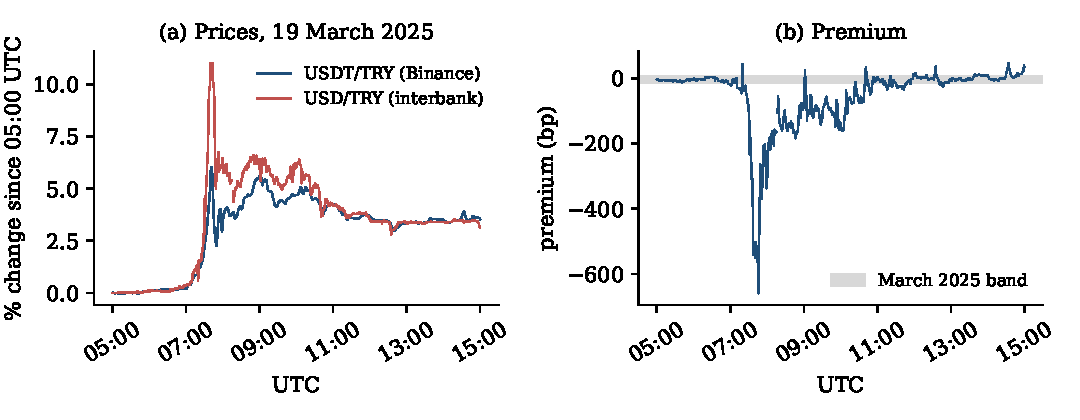
\includegraphics[width=\textwidth]{figures/emp_event.pdf}
\caption{\textbf{The 19 March 2025 lira shock.} Panel (a): percentage change in USDT/TRY (Binance VWAP) and interbank USD/TRY since 05:00 UTC. Panel (b): one-minute premium and the band estimated for March 2025.}
\label{fig:emp_event}
\end{figure}

\subsection{A regulatory event}

MASAK General Circular No.~29, published in the Official Gazette and effective on 28 June 2025, capped stablecoin transfers by users at USD 3,000 per day and USD 50,000 per month and imposed 48--72 hour holds on withdrawals, while exempting transfers for liquidity provision, market making and arbitrage when the funds are verified and controlled by the platform. The rule is directional. It constrains moving stablecoins \emph{out} of Turkish platforms, which is the arbitrage that closes a \emph{discount} (buy USDT cheaply in lira, move it abroad), and leaves the premium-side trade largely untouched. Remark~\ref{rem:carry} and Proposition~\ref{prop:policy} then predict a change on the discount side of the band only.

Table~\ref{tab:emp_masak} reports the lira market in the six months on either side of the circular, excluding the 19 March -- 30 April 2025 political shock. Effective capacity is stable in levels on both sides of the band, the sensitivity of the premium to order flow falls from $0.47$ to $0.32$, and the average premium falls from 7 bp to zero. Table~\ref{tab:emp_did} adds a control: USDT against the Mexican peso on the same exchange, measured against the interbank USD/MXN rate with the identical procedure, over the same window. The decline in the premium and in order-flow impact is shared with, and larger in, the control market, so it reflects common movements in dollar stablecoin markets over 2025. The circular's distinctive footprint is on the discount side: relative to the peso market, effective capacity below the band falls by $0.019$ (s.e.\ $0.0075$), while the premium-side difference is small and insignificant. In levels, discount-side capacity in the lira market stayed flat while it nearly doubled in the control market. The directional rule left a directional mark on the arbitrage technology, on the leg it constrained.

\begin{table}[t]
\centering
\caption{\textbf{The lira market around MASAK General Circular No.~29 (28 June 2025)}}
\label{tab:emp_masak}
\footnotesize
\resizebox{\ifdim\width>\textwidth\textwidth\else\width\fi}{!}{\begin{tabular}{lcc}
\toprule
 & Before & After \\
 & 28 Dec 2024 -- 27 Jun 2025 & 28 Jun -- 27 Dec 2025 \\
\midrule
$\kappa^+$ & $0.0060^{***}$ & $0.0087$ \\
 & $(0.0010)$ & $\Delta = 0.0028\;(0.0024)$ \\
$\kappa^-$ & $0.0099^{***}$ & $0.0091$ \\
 & $(0.0016)$ & $\Delta = -0.0008\;(0.0023)$ \\
$\beta$ & $0.473^{***}$ & $0.322$ \\
 & $(0.034)$ & $\Delta = -0.150^{***}\;(0.043)$ \\
Mean lower edge $\ell_m$ (bp) & -6.0 & -11.0 \\
Mean upper edge $u_m$ (bp) & 28.7 & 8.3 \\
Mean premium (bp) & 7.1 & -0.2 \\
5th / 95th percentile of premium (bp) & -26 / 41 & -29 / 29 \\
$N$ & 22,961 & 30,269 \\
\bottomrule
\end{tabular}
}
\begin{minipage}{0.95\textwidth}
\footnotesize\vspace{4pt}
\emph{Notes:} Specification~\eqref{eq:emp} with all slopes interacted with an indicator for the period after 28 June 2025; ``$\Delta$'' is the interaction coefficient. The pre-period excludes 19 March -- 30 April 2025. Band edges are averages of the monthly estimates. Month fixed effects; standard errors clustered by day.
\end{minipage}
\end{table}

\begin{table}[t]
\centering
\caption{\textbf{Difference-in-differences against USDT/MXN}}
\label{tab:emp_did}
\footnotesize
\resizebox{\ifdim\width>\textwidth\textwidth\else\width\fi}{!}{\begin{tabular}{lccc}
\toprule
 & Control (MXN): & Treated (TRY): & Difference-in- \\
 & change after & change after & differences \\
 & 28 Jun 2025 & 28 Jun 2025 & \\
\midrule
$\kappa^+$ & $0.0083$ & $0.0029$ & $-0.0054$ \\
 & $(0.0066)$ & & $(0.0078)$ \\
$\kappa^-$ & $0.0181^{**}$ & $-0.0006$ & $-0.0186^{**}$ \\
 & $(0.0071)$ & & $(0.0075)$ \\
$\beta$ & $-1.956^{***}$ & $-0.164$ & $1.792^{***}$ \\
 & $(0.155)$ & & $(0.155)$ \\
Mean premium (bp) & $-16.6^{***}$ & $-7.4$ & $9.2^{**}$ \\
 & $(4.9)$ & & $(4.2)$ \\
\midrule
$N$ (five-minute intervals) & 53,497 & 53,229 & 106,726 \\
\bottomrule
\end{tabular}
}
\begin{minipage}{0.95\textwidth}
\footnotesize\vspace{4pt}
\emph{Notes:} Stacked specification~\eqref{eq:emp} for USDT/TRY (treated) and USDT/MXN (control), 28 December 2024 -- 27 December 2025, excluding 19 March -- 30 April 2025 in both markets. Each market's premium is measured against its interbank USD rate (Dukascopy) with month-specific bands; order flow is standardized within market-month. All slopes are interacted with market and post-28-June indicators; market-by-month fixed effects. The mean-premium row uses daily averages with market fixed effects and week-clustered standard errors. Other standard errors are clustered by day.
\end{minipage}
\end{table}

\subsection{Integration over time}

Table~\ref{tab:emp_year} estimates~\eqref{eq:emp} by year. The primitive impact of standardized order flow falls from $1.04$ bp in 2024 to $0.43$ in 2025 and $0.25$ in 2026, the speed of arbitrage above the band rises from $0.0051$ to $0.0095$, and the standard deviation of the premium falls from $74$ to $16$ bp. Through Proposition~\ref{prop:stationary}, whose tail precision is $\lambda K/\sigma^2$, the tightening of the premium distribution reflects growing capacity. Over two and a half years the lira stablecoin market became markedly more integrated with the interbank market.

\paragraph{Band width and carry.} Remark~\ref{rem:carry} implies that the band widens with the interest differential, $u-\ell=c^++c^-+2(i-i^*)\tau$, where $\tau$ is the settlement horizon. Regressing the monthly band width on the monthly average difference between the CBRT one-week repo rate and the Federal funds target rate over 2024--2025 gives a slope of $290$ bp per unit of annual differential (Newey--West s.e.\ $144$, 24 months). The implied settlement horizon is $\hat\tau=\hat\gamma/2\approx 5$ days, with a wide confidence band, in the range of the bank-transfer, exchange-withdrawal and compliance delays that a cross-border round trip involves. The policy-rate differential moved only between 35 and 45 percentage points over the period, so this is a coarse calibration of the carry channel and a natural target for a multi-country design.

\begin{table}[t]
\centering
\caption{\textbf{Estimates by year}}
\label{tab:emp_year}
\footnotesize
\resizebox{\ifdim\width>\textwidth\textwidth\else\width\fi}{!}{\begin{tabular}{lccccc}
\toprule
 Year & $\beta$ & $\kappa^+$ & $\kappa^-$ & Median band width (bp) & SD of premium (bp) \\
\midrule
2024 & $1.041^{***}$ & $0.0051^{***}$ & $0.0050^{***}$ & 47 & 74.1 \\
 & $(0.055)$ & $(0.0014)$ & $(0.0011)$ & & \\
2025 & $0.431^{***}$ & $0.0065^{***}$ & $0.0212^{**}$ & 20 & 24.5 \\
 & $(0.040)$ & $(0.0015)$ & $(0.0091)$ & & \\
2026 & $0.249^{***}$ & $0.0095^{***}$ & $0.0094^{***}$ & 30 & 16.4 \\
 & $(0.018)$ & $(0.0015)$ & $(0.0020)$ & & \\
\bottomrule
\end{tabular}
}
\begin{minipage}{0.95\textwidth}
\footnotesize\vspace{4pt}
\emph{Notes:} Specification~\eqref{eq:emp} with year-specific slopes, month fixed effects and month-specific bands. Standard errors clustered by day.
\end{minipage}
\end{table}

\subsection{Robustness}

Table~\ref{tab:emp_robust} re-estimates the main specification at one- and fifteen-minute frequencies, with last-trade prices in place of VWAPs, without the 19 March -- 30 April 2025 window, with quarterly bands, and with 10\% trimming. Reversion outside the band is positive and significant in every specification and scales with the sampling interval, the fifteen-minute speeds being about three times the five-minute ones. The business-hours increase in $\kappa^+$ is significant at 1\% throughout. Inside the band, reversion is zero at the one- and five-minute frequencies with monthly bands; at the fifteen-minute frequency and with quarterly bands, which place some out-of-band observations inside the band, it is between one fifth and two fifths of the speed outside the band.

\begin{table}[t]
\centering
\caption{\textbf{Robustness}}
\label{tab:emp_robust}
\footnotesize
\resizebox{\ifdim\width>\textwidth\textwidth\else\width\fi}{!}{\begin{tabular}{lccccc}
\toprule
 & $\beta$ & $\kappa^+$ & $\kappa^-$ & In-band reversion & $\kappa^+_{BH}-\kappa^+_{off}$ \\
\midrule
Baseline: 5-min, VWAP, monthly bands, 5\% trimming & $0.604^{***}$ & $0.0054^{***}$ & $0.0085^{***}$ & $-0.0006$ & $0.0079^{***}$ \\
 & $(0.030)$ & $(0.0013)$ & $(0.0025)$ & $(0.0007)$ & $(0.0014)$ \\
1-minute frequency & $0.342^{***}$ & $0.0011^{***}$ & $0.0036^{***}$ & $-0.0005^{*}$ & $0.0014^{***}$ \\
 & $(0.013)$ & $(0.0003)$ & $(0.0009)$ & $(0.0003)$ & $(0.0003)$ \\
15-minute frequency & $1.116^{***}$ & $0.0187^{***}$ & $0.0243^{***}$ & $0.0039^{**}$ & $0.0278^{***}$ \\
 & $(0.067)$ & $(0.0028)$ & $(0.0070)$ & $(0.0018)$ & $(0.0045)$ \\
Last-trade price instead of VWAP & $0.643^{***}$ & $0.0056^{***}$ & $0.0091^{***}$ & $-0.0006$ & $0.0080^{***}$ \\
 & $(0.032)$ & $(0.0013)$ & $(0.0025)$ & $(0.0007)$ & $(0.0015)$ \\
Excluding 19 Mar--30 Apr 2025 & $0.598^{***}$ & $0.0054^{***}$ & $0.0062^{***}$ & $-0.0005$ & $0.0080^{***}$ \\
 & $(0.029)$ & $(0.0013)$ & $(0.0010)$ & $(0.0007)$ & $(0.0015)$ \\
Quarterly bands & $0.604^{***}$ & $0.0044^{***}$ & $0.0130^{***}$ & $0.0017^{***}$ & $0.0062^{***}$ \\
 & $(0.030)$ & $(0.0011)$ & $(0.0046)$ & $(0.0006)$ & $(0.0015)$ \\
10\% trimming & $0.604^{***}$ & $0.0042^{***}$ & $0.0098^{***}$ & $-0.0002$ & $0.0070^{***}$ \\
 & $(0.030)$ & $(0.0011)$ & $(0.0034)$ & $(0.0007)$ & $(0.0014)$ \\
\bottomrule
\end{tabular}
}
\begin{minipage}{0.95\textwidth}
\footnotesize\vspace{4pt}
\emph{Notes:} Each row re-estimates columns (2)--(4) of Table~\ref{tab:emp_main}. ``In-band reversion'' is the coefficient on $-(b_{t-1}-m_m)\mathbb 1\{\text{in band}\}$ in column (3). The last column is the business-hours interaction on $\kappa^+$ in column (4). Reversion coefficients are per sampling interval. Standard errors clustered by day.
\end{minipage}
\end{table}

%=====================================================================
\section{Conclusion}\label{sec:conclusion}
%=====================================================================

The law of one price for dollar stablecoins holds as far as arbitrage capacity allows. A per-unit cost and a finite capacity turn the local premium into a threshold diffusion, separate what volume reveals (demand) from what the premium reveals (capacity), bound the market's ability to absorb demand by an arbitrage throughput limit, and filter which local information reaches the global price.

In the lira stablecoin market, premia inside a band of about 30 bp do not revert, arbitrage switches on outside the band and runs four to five times faster when banks are open, large trades lean against the dislocations that small trades open, a rule on outbound transfers slowed the arbitrage leg it constrained, and the interbank market sets the price that the stablecoin market follows. The same design applies to the naira, peso and won markets, where different capital-control regimes and interest differentials imply different bands for the same demand, and to direct measures of capacity such as exchange withdrawal flows. Whether a local market helps discover the dollar's value, or pays for access to it, is a question its premium and order flow can answer.

\paragraph{Data and code availability.} All data are public: Binance spot candles (\url{https://data.binance.vision}) and Dukascopy interbank candles. Code that downloads the data and reproduces every table and figure is available from the author upon request.

\clearpage
\singlespacing
\begin{thebibliography}{99}
\setlength{\itemsep}{2pt}

\bibitem[Aldasoro et al.(2026)]{aldasoro2026stablecoin}
Aldasoro, I., P. Beltran, and F. Grinberg (2026). Stablecoin inflows and spillovers to FX markets. IMF Working Paper 26/56.

\bibitem[Balke and Fomby(1997)]{balke1997threshold}
Balke, N.~S. and T.~B. Fomby (1997). Threshold cointegration. \emph{International Economic Review} 38(3), 627--645.

\bibitem[Brunnermeier and Pedersen(2009)]{brunnermeier2009market}
Brunnermeier, M.~K. and L.~H. Pedersen (2009). Market liquidity and funding liquidity. \emph{Review of Financial Studies} 22(6), 2201--2238.

\bibitem[Cont et al.(2014)]{cont2014price}
Cont, R., A. Kukanov, and S. Stoikov (2014). The price impact of order book events. \emph{Journal of Financial Econometrics} 12(1), 47--88.

\bibitem[Du et al.(2018)]{du2018deviations}
Du, W., A. Tepper, and A. Verdelhan (2018). Deviations from covered interest rate parity. \emph{Journal of Finance} 73(3), 915--957.

\bibitem[Duffie(2010)]{duffie2010presidential}
Duffie, D. (2010). Presidential address: Asset price dynamics with slow-moving capital. \emph{Journal of Finance} 65(4), 1237--1267.

\bibitem[Dumas(1992)]{dumas1992dynamic}
Dumas, B. (1992). Dynamic equilibrium and the real exchange rate in a spatially separated world. \emph{Review of Financial Studies} 5(2), 153--180.

\bibitem[Fiedler(1973)]{fiedler1973algebraic}
Fiedler, M. (1973). Algebraic connectivity of graphs. \emph{Czechoslovak Mathematical Journal} 23(2), 298--305.

\bibitem[Gonzalo and Granger(1995)]{gonzalo1995estimation}
Gonzalo, J. and C. Granger (1995). Estimation of common long-memory components in cointegrated systems. \emph{Journal of Business \& Economic Statistics} 13(1), 27--35.

\bibitem[Griffin and Shams(2020)]{griffin2020untethered}
Griffin, J.~M. and A. Shams (2020). Is Bitcoin really untethered? \emph{Journal of Finance} 75(4), 1913--1964.

\bibitem[Gromb and Vayanos(2002)]{gromb2002equilibrium}
Gromb, D. and D. Vayanos (2002). Equilibrium and welfare in markets with financially constrained arbitrageurs. \emph{Journal of Financial Economics} 66(2--3), 361--407.

\bibitem[Hansen(1996)]{hansen1996inference}
Hansen, B.~E. (1996). Inference when a nuisance parameter is not identified under the null hypothesis. \emph{Econometrica} 64(2), 413--430.

\bibitem[Hansen(2000)]{hansen2000sample}
Hansen, B.~E. (2000). Sample splitting and threshold estimation. \emph{Econometrica} 68(3), 575--603.

\bibitem[Hansen and Seo(2002)]{hansen2002testing}
Hansen, B.~E. and B. Seo (2002). Testing for two-regime threshold cointegration in vector error-correction models. \emph{Journal of Econometrics} 110(2), 293--318.

\bibitem[Hasbrouck(1995)]{hasbrouck1995one}
Hasbrouck, J. (1995). One security, many markets: Determining the contributions to price discovery. \emph{Journal of Finance} 50(4), 1175--1199.

\bibitem[Hautsch et al.(2024)]{hautsch2024building}
Hautsch, N., C. Scheuch, and S. Voigt (2024). Building trust takes time: Limits to arbitrage for blockchain-based assets. \emph{Review of Finance} 28(4), 1345--1381.

\bibitem[Hu and Zhang(2023)]{hu2023competition}
Hu, J. and A.~L. Zhang (2023). Competition in the cryptocurrency exchange market. Working paper, University of Chicago.

\bibitem[Lehar et al.(2024)]{lehar2024fragmentation}
Lehar, A., C.~A. Parlour, and M. Zoican (2024). Fragmentation and optimal liquidity supply on decentralized exchanges. Working paper, arXiv:2307.13772.

\bibitem[Lyons and Viswanath-Natraj(2023)]{lyons2023stablecoins}
Lyons, R.~K. and G. Viswanath-Natraj (2023). What keeps stablecoins stable? \emph{Journal of International Money and Finance} 131, 102777.

\bibitem[Ma et al.(2025)]{ma2025stablecoin}
Ma, Y., Y. Zeng, and A.~L. Zhang (2025). Stablecoin runs and the centralization of arbitrage. \emph{Review of Financial Studies}, forthcoming. NBER Working Paper 33882.

\bibitem[Makarov and Schoar(2020)]{makarov2020trading}
Makarov, I. and A. Schoar (2020). Trading and arbitrage in cryptocurrency markets. \emph{Journal of Financial Economics} 135(2), 293--319.

\bibitem[Mitchell et al.(2007)]{mitchell2007slow}
Mitchell, M., L.~H. Pedersen, and T. Pulvino (2007). Slow moving capital. \emph{American Economic Review} 97(2), 215--220.

\bibitem[Obstfeld and Taylor(1997)]{obstfeld1997nonlinear}
Obstfeld, M. and A.~M. Taylor (1997). Nonlinear aspects of goods-market arbitrage and adjustment: Heckscher's commodity points revisited. \emph{Journal of the Japanese and International Economies} 11(4), 441--479.

\bibitem[Shleifer and Vishny(1997)]{shleifer1997limits}
Shleifer, A. and R.~W. Vishny (1997). The limits of arbitrage. \emph{Journal of Finance} 52(1), 35--55.

\end{thebibliography}

\newpage
\onehalfspacing
\appendix
\section{Proofs}\label{app:proofs}

\paragraph{Proof of Proposition~\ref{prop:policy}.}
$\Pi(\cdot;b)$ is continuous and strictly concave on $\mathbb R$: it is strictly concave on each half-line, and at $a=0$ its left derivative $b+c^-$ exceeds its right derivative $b-c^+$, so the kink is concave. Hence the maximizer is unique and is characterized by $0\in\partial\Pi(a^*;b)$. At $a=0$ the superdifferential is $[b-c^+,\,b+c^-]$, which contains $0$ if and only if $-c^-\le b\le c^+$. If $b>c^+$, the right derivative at zero is positive, so $a^*>0$ solves $b-c^+-a/K^+=0$, i.e.\ $a^*=K^+(b-c^+)$. If $b<-c^-$, the left derivative at zero is negative, so $a^*<0$ solves $b+c^--a/K^-=0$, i.e.\ $a^*=K^-(b+c^-)=-K^-(-b-c^-)$. Combining the cases gives~\eqref{eq:policy}. \qed

\paragraph{Proof of Proposition~\ref{prop:reversion}.}
(a) With $q\equiv0$ and $b_s\in(-c^-,c^+)$ for $s<\tau$, the drift vanishes, so $b_{t\wedge\tau}=b_0+\sigma W_{t\wedge\tau}$ is a stopped Brownian motion and hence a martingale. The expected exit time of $b_0+\sigma W$ from $(-c^-,c^+)$ solves $\frac{\sigma^2}{2}u''=-1$ with $u(-c^-)=u(c^+)=0$, whose solution is $u(b_0)=(c^+-b_0)(b_0+c^-)/\sigma^2$.
(b) With $\sigma=0$ and $b>c^+$, $\dot b=-\kappa^+(b-c^+)$. The solution $b_t=c^++(b_0-c^+)e^{-\kappa^+t}$ stays above $c^+$ for all $t$, so the linear dynamics remain valid. The excess halves when $e^{-\kappa^+t}=1/2$.
(c) For $b>c^+$, $\rho(b)=\kappa^+(b-c^+)/b=\kappa^+(1-c^+/b)$, which is increasing in $b$ and tends to $\kappa^+$. On the band $\rho=0$. The case $b<-c^-$ is symmetric. \qed

\paragraph{Proof of Proposition~\ref{prop:impact}.}
(a) Let $q>0$ and $\sigma=0$, so $\dot b=f(b)\equiv\beta q+\mu(b)$. The function $f$ is continuous and strictly positive for $b\le c^+$, strictly decreasing on $(c^+,\infty)$, and has a unique zero at $b^*=c^++\beta q/\kappa^+$. Since $f>0$ below $b^*$ and $f<0$ above it, every trajectory converges monotonically to $b^*$. The case $q<0$ is symmetric. If $q=0$, $f$ vanishes on the band and the argument of Proposition~\ref{prop:reversion}(b) applies outside it.
(b) Differentiate $b^*$.
(c) At the steady state $\dot b=0$, so $\beta q=\lambda a^*$. \qed

\paragraph{Proof of Corollary~\ref{cor:equivalence}.}
Immediate from Proposition~\ref{prop:impact}(a) applied to each market. \qed

\paragraph{Proof of Proposition~\ref{prop:depletion}.}
Write $x_t=b_t-c$ and $a_t=K_t(x_t)_+\ge0$. The system is
\[
\dot x=\beta q-\lambda a,\qquad \dot K=\xi(\bar K-K)-\chi a .
\]
The set $\{K>0\}$ is forward invariant: at $K=0$, $a=0$ and $\dot K=\xi\bar K>0$.

(a) A steady state requires $\lambda a=\beta q>0$, so $x>0$ and $a=K x=\beta q/\lambda$. Then $\dot K=0$ gives $K^*=\bar K-\chi\beta q/(\xi\lambda)=\bar K(1-q/q_{crit})$, which is positive if and only if $q<q_{crit}$, and $x^*=\beta q/(\lambda K^*)$. In the region $x>0$ the Jacobian is
\[
J=\begin{pmatrix}-\lambda K & -\lambda x\\ -\chi K & -\xi-\chi x\end{pmatrix},
\qquad \operatorname{tr}J<0,\qquad \det J=\lambda K(\xi+\chi x)-\lambda\chi Kx=\lambda\xi K>0,
\]
so both eigenvalues have negative real parts at $(x^*,K^*)$, which establishes local asymptotic stability. Differentiating $b^*=c+\beta q/(\lambda\bar K(1-q/q_{crit}))$ gives $\partial b^*/\partial q=\beta/(\lambda\bar K)\cdot\big[(1-q/q_{crit})+q/q_{crit}\big]/(1-q/q_{crit})^2=\beta/(\lambda\bar K(1-q/q_{crit})^2)$, which is increasing and convex on $[0,q_{crit})$ and diverges as $q\uparrow q_{crit}$.

(b) Integrating the capacity equation over $[0,T]$ and using $K_T>0$ and $K_t\ge0$,
\[
\chi\int_0^Ta_t\,dt = \xi\bar KT-\xi\int_0^TK_tdt-(K_T-K_0)\le \xi\bar KT+K_0 .
\]
Hence $\int_0^Ta_tdt\le\bar aT+K_0/\chi$. Integrating the premium equation,
\[
x_T=x_0+\beta qT-\lambda\int_0^Ta_tdt\ \ge\ x_0-\frac{\lambda K_0}{\chi}+(\beta q-\lambda\bar a)T .
\]
Dividing by $T$ and letting $T\to\infty$ gives $\liminf x_T/T\ge\beta q-\lambda\bar a=\beta(q-q_{crit})$. If $q>q_{crit}$ this is positive, so no steady state can exist. \qed

\paragraph{Proof of Proposition~\ref{prop:discovery}.}
After the shock, $b_0=\delta$ and $\dot b=-\lambda a^*(b)$, with $\dot p^G=\lambda_Ga^*(b)$. If $\delta\le c^+$, $a^*=0$ for all $t$ and $p^G$ does not move. If $\delta>c^+$, Proposition~\ref{prop:reversion}(b) gives $b_t-c^+=(\delta-c^+)e^{-\lambda K^+t}$. Since $\dot p^G=\lambda_Ga^*=-\frac{\lambda_G}{\lambda}\dot b$,
\[
p^G_h-p^G_0=\omega\,(b_0-b_h)=\omega(\delta-c^+)\big(1-e^{-\lambda K^+h}\big).
\]
Dividing by $\delta$ gives $S_h(\delta)$, and parts (a)--(c) follow by inspection. \qed

\paragraph{Proof of Proposition~\ref{prop:stationary}.}
For a one-dimensional diffusion $db=\mu(b)dt+\sigma dW$ with Lipschitz drift, the speed measure has density $m(b)=\frac{2}{\sigma^2}\exp\!\big(\frac{2}{\sigma^2}\int_0^b\mu(x)dx\big)$. The process is positive recurrent, with stationary density proportional to $m$, whenever $m$ is integrable and the scale function diverges at $\pm\infty$. Here $\int_0^b\mu=0$ on the band, $-\frac{\kappa^+}{2}(b-c^+)^2$ for $b>c^+$, and $-\frac{\kappa^-}{2}(b+c^-)^2$ for $b<-c^-$. This gives~\eqref{eq:density}, which is integrable. The scale density $1/m$ grows like a Gaussian reciprocal, so the scale function diverges at both ends. For the constant, use $\int_0^\infty e^{-\theta x^2}dx=\frac12\sqrt{\pi/\theta}$ with $\theta=\kappa^\pm/\sigma^2$. Part (a) follows by integrating the plateau. For part (b), $\int_{-c^-}^{c^+}b\,db=\frac{(c^+)^2-(c^-)^2}{2}$ and $\int_{c^+}^\infty b\,e^{-\theta(b-c^+)^2}db=c^+\cdot\frac12\sqrt{\pi/\theta}+\frac{1}{2\theta}$, with $\frac{1}{2\theta}=\frac{\sigma^2}{2\kappa^+}$; the lower tail is symmetric with the opposite sign. \qed

\paragraph{Proof of Proposition~\ref{prop:network}.}
Since $P$ is a projection and $P\mathbf 1=0$, $z=Pp$ satisfies $dz=-P F(p)\,dt+P\Sigma\,dW$, where $F_i(p)=\sum_jw_{ij}\phi_{c_{ij}}(p_i-p_j)$. By Itô's lemma, $V(z)=\frac12\|z\|^2$ has generator
\[
\mathcal LV = -z'F(p)+\tfrac12\operatorname{tr}(P\Sigma\Sigma'P),
\]
where we used $z'P=z'$. By symmetry of $w$ and oddness of $\phi$,
\[
z'F(p)=\sum_i\sum_jw_{ij}z_i\phi_{c_{ij}}(p_i-p_j)=\sum_{i<j}w_{ij}(z_i-z_j)\phi_{c_{ij}}(p_i-p_j)=\sum_{i<j}w_{ij}(p_i-p_j)\phi_{c_{ij}}(p_i-p_j),
\]
since $z_i-z_j=p_i-p_j$. For any $x$ and $c>0$, $x\phi_c(x)\ge\frac12x^2-\frac12c^2$. This holds trivially for $|x|\le c$; for $|x|>c$, $x\phi_c(x)=x^2-c|x|\ge x^2-\frac12(x^2+c^2)$. Therefore
\[
z'F(p)\ge\tfrac12\sum_{i<j}w_{ij}(p_i-p_j)^2-\tfrac12\sum_{i<j}w_{ij}c_{ij}^2=\tfrac12z'L_wz-\tfrac12\sum_{i<j}w_{ij}c_{ij}^2 .
\]
Since $z\perp\mathbf 1$, the Courant--Fischer theorem gives $z'L_wz\ge\lambda_2(L_w)\|z\|^2=2\lambda_2(L_w)V$. Thus
\[
\mathcal LV\le-\lambda_2(L_w)V+C,\qquad C\equiv\tfrac12\sum_{i<j}w_{ij}c_{ij}^2+\tfrac12\operatorname{tr}(P\Sigma\Sigma'P).
\]
By Dynkin's formula with a standard localization argument (the drift is Lipschitz, so all moments are finite), $\frac{d}{dt}\E V(z_t)\le-\lambda_2\E V(z_t)+C$. Gr\"onwall's inequality then gives $\E V(z_t)\le e^{-\lambda_2t}\E V(z_0)+C/\lambda_2$, which yields the bound. If the network is disconnected, take two components $A$ and $B$. The difference between their average prices has no drift, because arbitrage within each component preserves its average. If the noise is non-degenerate across components, that difference is a Brownian motion with positive variance rate, so its second moment, and hence $\E V$, grows linearly. \qed

\paragraph{Proof of Corollary~\ref{cor:hub}.}
(a) The Laplacian of the star $K_{1,N-1}$ with weight $w$ has eigenvalues $0$, $w$ (multiplicity $N-2$) and $Nw$, so $\lambda_2=w$. For any non-complete graph, \citet{fiedler1973algebraic} shows that algebraic connectivity is bounded above by vertex connectivity. Every tree on $N\ge3$ vertices has vertex connectivity one, so $\lambda_2\le w$ for every spanning tree with weight $w$, and the star attains the bound.
(b) Deleting the hub removes all edges. Deleting a leaf leaves a star on $N-1$ vertices, whose algebraic connectivity is again $w$ for $N-1\ge3$ (for $N-1=2$ it is $2w$). Unbounded dispersion follows from the last part of Proposition~\ref{prop:network}.
(c) The complete graph $K_N$ with weight $w$ has Laplacian $w(NI-\mathbf 1\mathbf 1')$, with eigenvalues $0$ and $Nw$ (multiplicity $N-1$). Removing a vertex leaves $K_{N-1}$. \qed


\section{Further theoretical results}\label{app:theory}

\subsection{The stationary distribution of the premium}

When order flow has mean zero and is short-lived relative to arbitrage, its effect is absorbed into the diffusion term. The premium then has an explicit stationary law.

\begin{proposition}[Stationary distribution]\label{prop:stationary}
Let $q\equiv0$. The premium process~\eqref{eq:sde} is positive recurrent with unique stationary density
\begin{equation}\label{eq:density}
\pi(b) = \frac{1}{Z}
\begin{cases}
\exp\!\Big[-\dfrac{\lambda K^+}{\sigma^2}(b-c^+)^2\Big], & b>c^+,\\[8pt]
1, & -c^-\le b\le c^+,\\[4pt]
\exp\!\Big[-\dfrac{\lambda K^-}{\sigma^2}(b+c^-)^2\Big], & b<-c^-,
\end{cases}
\end{equation}
with normalizing constant
\[
Z = c^++c^- + s^+ + s^-,\qquad s^\pm \equiv \frac12\sqrt{\frac{\pi\sigma^2}{\lambda K^\pm}} .
\]
Consequently:
\begin{enumerate}[label=(\alph*)]
\item The stationary probability that the premium lies inside the band is $(c^++c^-)/Z$.
\item The stationary mean premium is
\[
\E_\pi[b] = \frac{1}{Z}\left[\frac{(c^+)^2-(c^-)^2}{2} + c^+s^+ - c^-s^- + \frac{\sigma^2}{2\lambda K^+} - \frac{\sigma^2}{2\lambda K^-}\right],
\]
which is non-zero whenever frictions or capacities are asymmetric, even though order flow has mean zero.
\end{enumerate}
\end{proposition}

The density in~\eqref{eq:density} has a distinctive shape: a flat plateau whose width is the band, joined continuously to half-Gaussian tails whose precision $\lambda K^\pm/\sigma^2$ measures capacity relative to noise. Figure~\ref{fig:density} compares it with a long simulated path. Part (b) cautions against reading a persistent average premium as excess demand. If it is harder to move dollars out of the country than in ($c^+>c^-$ or $K^+<K^-$), the premium is positive on average even when order flow is balanced.

\begin{figure}[t]
\centering
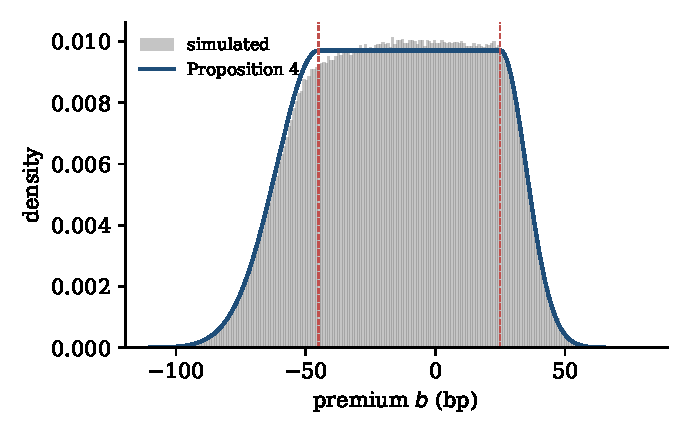
\includegraphics[width=0.62\textwidth]{figures/fig2_density.pdf}
\caption{\textbf{Stationary distribution of the premium.} Asymmetric design with $c^+=25$, $c^-=45$ bp, $\lambda K^+=0.08$, $\lambda K^-=0.03$ per minute and $\sigma=4$ bp$/\sqrt{\text{min}}$. The histogram is a simulated path of $2\times10^6$ minutes; the solid line is the closed form~\eqref{eq:density}. Dashed lines mark the band. The theoretical probability of being inside the band is $0.680$, against $0.688$ in the simulation (the small gap reflects Euler discretization at the boundary).}
\label{fig:density}
\end{figure}

\subsection{Illustrations of Propositions~\ref{prop:depletion} and~\ref{prop:discovery}}

\begin{figure}[t]
\centering
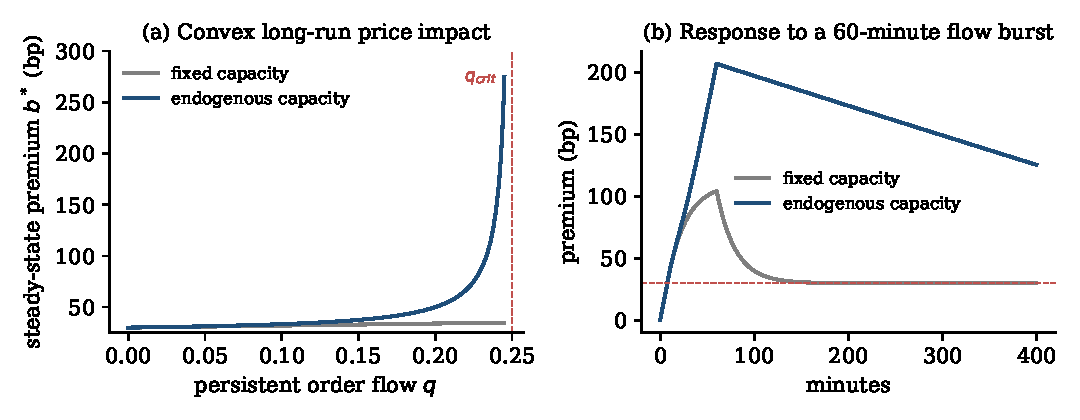
\includegraphics[width=\textwidth]{figures/fig3_capacity.pdf}
\caption{\textbf{Capacity depletion.} Parameters: $\beta=\lambda=1$, $\bar K=0.05$, $\xi=0.01$, $\chi=0.002$, $c=30$ bp, so $q_{crit}=0.25$. Panel (a): steady-state premium against persistent order flow, with fixed capacity (grey) and endogenous capacity (Proposition~\ref{prop:depletion}). Panel (b): response to order flow $q=4$ for 60 minutes. With fixed capacity the post-burst half-life of the excess premium is $13.9$ minutes, equal to $\ln2/(\lambda\bar K)$; with endogenous capacity it is $370$ minutes.}
\label{fig:capacity}
\end{figure}

\begin{figure}[t]
\centering
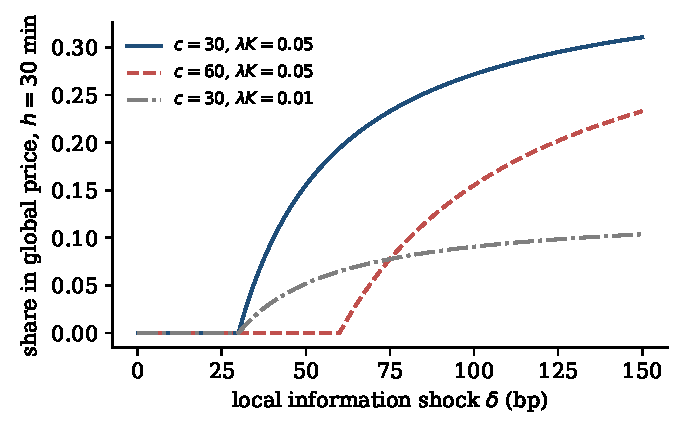
\includegraphics[width=0.62\textwidth]{figures/fig4_discovery.pdf}
\caption{\textbf{Transmission of local information to the global price.} Fraction of a local information shock of size $\delta$ incorporated into the global price within $h=30$ minutes (Proposition~\ref{prop:discovery}), with $\omega=0.5$, for different frictions $c$ and capacities $\lambda K$.}
\label{fig:discovery}
\end{figure}

\subsection{Networks of venues}\label{sec:network}
%=====================================================================

Stablecoins trade on many venues at once: several local exchanges, peer-to-peer platforms, and global order books. We now let $N\ge3$ venues with log prices $p_t=(p_{1t},\dots,p_{Nt})'$ be connected by pairwise threshold arbitrage. Let $w_{ij}=w_{ji}\ge0$ be the capacity-scaled arbitrage intensity on link $\{i,j\}$, and $c_{ij}=c_{ji}>0$ its friction. Let $\phi_c(x)\equiv\sgn(x)\pos{|x|-c}$ denote the soft-threshold function. Prices follow
\begin{equation}\label{eq:network}
dp_{it} = -\sum_{j\ne i} w_{ij}\,\phi_{c_{ij}}(p_{it}-p_{jt})\,dt + (\Sigma\,dW_t)_i ,
\end{equation}
where $\Sigma$ is an $N\times N$ volatility matrix that also absorbs mean-zero order-flow shocks. Let $L_w$ be the weighted graph Laplacian of $(w_{ij})$, and let $\lambda_2(L_w)$ be its second-smallest eigenvalue, the \emph{algebraic connectivity} of the arbitrage network \citep{fiedler1973algebraic}. The network is connected if and only if $\lambda_2(L_w)>0$. Cross-venue disagreement is measured by $z_t=Pp_t$ with $P=I-\frac1N\mathbf{1}\mathbf{1}'$ and $V(z)=\frac12\|z\|^2$.

\begin{proposition}[Dispersion and connectivity]\label{prop:network}
If the arbitrage network is connected, then
\[
\limsup_{t\to\infty}\E[V(z_t)] \;\le\; \frac{\tfrac12\sum_{i<j}w_{ij}c_{ij}^2 + \tfrac12\operatorname{tr}(P\Sigma\Sigma'P)}{\lambda_2(L_w)} .
\]
If the network is disconnected, $\E[V(z_t)]$ grows linearly in $t$ whenever the noise is non-degenerate across components.
\end{proposition}

The bound has two terms in the numerator. The first is the dispersion that frictions tolerate inside the bands; the second is the dispersion generated by noise. The denominator is the network's ability to pull prices together. Long-run dispersion therefore depends on capacity only through $\lambda_2$, which depends on the \emph{topology} of the network as well as on the level of capacity. Two corollaries follow.

\begin{corollary}[Centralized arbitrage: efficient and fragile]\label{cor:hub}
Suppose links are costly, so that the arbitrage network is a spanning tree, and each link has the same intensity $w$.
\begin{enumerate}[label=(\alph*)]
\item The star network, in which a single hub venue is linked to every other venue, attains $\lambda_2(L_w)=w$. This is the maximum over all spanning trees, so the hub structure minimizes the dispersion bound among minimal networks.
\item If the hub fails, all links vanish, the remaining $N-1$ venues are mutually disconnected, and dispersion grows without bound. Removing any single non-hub venue leaves $\lambda_2=w$ unchanged.
\item By contrast, in the complete network with intensity $w$ on every link, $\lambda_2=Nw$, and removing any venue leaves $\lambda_2=(N-1)w$.
\end{enumerate}
\end{corollary}

Corollary~\ref{cor:hub} formalizes a trade-off. When maintaining an arbitrage link is costly (accounts, banking relationships and transfer rails must be set up for each pair of venues), arbitrage naturally concentrates in a hub. In crypto the hub is typically the largest global exchange or a dominant market maker \citep{hu2023competition}. The hub maximizes integration in normal times, but its failure disconnects the market. This mirrors, across secondary-market venues, the primary-market trade-off documented by \citet{ma2025stablecoin}, and it predicts that the dispersion of local stablecoin prices should spike when a hub venue suspends withdrawals or a hub arbitrageur exits, by much more than when a peripheral venue does.


\section{Monte Carlo evidence on the estimator}\label{sec:mc}
%=====================================================================

This section shows that the estimator recovers the structural parameters at realistic sample sizes and that linear models are misleading when the data are generated by threshold arbitrage. Units are basis points and minutes. The baseline design has $c^\pm=30$ bp, $\kappa^\pm=0.05$ per minute (half-life 14 minutes), $\beta=1$, $\sigma=4$ bp$/\sqrt{\text{min}}$, and order flow following a standardized AR(1) with autocorrelation $0.9$. The asymmetric design has $c^+=20$, $c^-=50$, $\kappa^+=0.08$ and $\kappa^-=0.02$. The low-capacity design sets $\kappa^\pm=0.015$. Each replication has $T=20{,}000$ observations, about two weeks of minute data, and there are $200$ replications per design. Thresholds are profiled over a grid with $2.5$ bp spacing.

\begin{table}[t]
\centering
\caption{\textbf{Monte Carlo: recovery of structural parameters}}
\label{tab:mc}
\small
\begin{tabular}{lccccc}
\toprule
 & $c^+$ & $c^-$ & $\kappa^+=\lambda K^+$ & $\kappa^-=\lambda K^-$ & $\beta$ \\
\midrule
\multicolumn{6}{l}{\textit{Symmetric design}} \\
True & 30.0 & 30.0 & 0.050 & 0.050 & 1.000 \\
Median estimate & 30.0 & 30.0 & 0.050 & 0.051 & 0.999 \\
RMSE & 2.5 & 2.7 & 0.007 & 0.007 & 0.029 \\
Linear ECM $\hat\kappa$ & \multicolumn{4}{c}{0.0147} & 0.964 \\
\addlinespace
\multicolumn{6}{l}{\textit{Asymmetric design}} \\
True & 20.0 & 50.0 & 0.080 & 0.020 & 1.000 \\
Median estimate & 20.0 & 50.0 & 0.081 & 0.020 & 0.999 \\
RMSE & 2.0 & 6.8 & 0.011 & 0.004 & 0.028 \\
Linear ECM $\hat\kappa$ & \multicolumn{4}{c}{0.0105} & 0.963 \\
\addlinespace
\multicolumn{6}{l}{\textit{Low capacity design}} \\
True & 30.0 & 30.0 & 0.015 & 0.015 & 1.000 \\
Median estimate & 30.0 & 30.0 & 0.016 & 0.015 & 0.999 \\
RMSE & 8.5 & 8.9 & 0.004 & 0.004 & 0.028 \\
Linear ECM $\hat\kappa$ & \multicolumn{4}{c}{0.0075} & 0.991 \\
\addlinespace
\bottomrule
\end{tabular}

\begin{minipage}{0.92\textwidth}
\footnotesize
\vspace{4pt}
\emph{Notes:} $200$ replications of $T=20{,}000$ one-minute observations per design. ``Median estimate'' and ``RMSE'' refer to the profiled least-squares estimator of~\eqref{eq:emp}. ``Linear ECM'' reports the median reversion coefficient (first four columns) and order-flow coefficient (last column) from $\Delta b_{t+1}=\alpha+\beta\,\mathit{OFI}_t-\kappa b_t+\varepsilon_{t+1}$.
\end{minipage}
\end{table}

Table~\ref{tab:mc} reports the results. The thresholds are estimated with an RMSE of 2--3 bp in the baseline. Capacity-scaled speeds and order-flow impact are essentially unbiased. Asymmetries in both the band and capacity are recovered. In the low-capacity design the premium spends more time far outside the band, so its edges are visited less sharply and the thresholds are estimated less precisely, though still without bias. The implied long-run impact multipliers $\beta/\kappa^+$ have median estimates of $19.8$, $12.3$ and $63.9$ against true values of $20.0$, $12.5$ and $66.7$. The capacity differences that Corollary~\ref{cor:equivalence} says are hidden in raw premia are therefore recoverable from the joint dynamics of premia and order flow.

The linear error-correction model performs poorly. Its reversion coefficient is $0.015$ in the baseline, less than a third of the true speed outside the band, and it implies a half-life of 47 minutes instead of 14. In the asymmetric design it averages two very different speeds into a single number. Reading the linear coefficient as a measure of arbitrage capacity, and $\beta/\hat\kappa$ as long-run impact, would overstate the long-run price impact of order flow by a factor of about two (low-capacity design) to more than three (baseline).

\begin{table}[t]
\centering
\caption{\textbf{Reversion speed by size of dislocation (baseline design)}}
\label{tab:bins}
\small
\begin{tabular}{lcccccc}
\toprule
$|b_t|$ (bp) & [0,10) & [10,20) & [20,30) & [30,45) & [45,60) & [60,90) \\
\midrule
Reversion speed per minute & -0.0027 & -0.0011 & -0.0003 & 0.0101 & 0.0212 & 0.0273 \\
Implied half-life (min) & $\infty$ & $\infty$ & $\infty$ & 68 & 33 & 25 \\
Share of observations & 0.175 & 0.182 & 0.190 & 0.271 & 0.143 & 0.039 \\
\bottomrule
\end{tabular}

\begin{minipage}{0.92\textwidth}
\footnotesize
\vspace{4pt}
\emph{Notes:} Simulated path of $5\times10^5$ minutes. Within each bin of $|b_t|$, the table reports the slope from regressing $-\Delta b_{t+1}\,\sgn(b_t)$ on $|b_t|$ and $\mathit{OFI}_t\,\sgn(b_t)$ without an intercept, and the implied half-life $\ln2/\text{slope}$ (reported as $\infty$ when the slope is not positive). The band is $[-30,30]$ bp.
\end{minipage}
\end{table}

Table~\ref{tab:bins} implements test T2 on a long simulated path. Reversion is absent inside the band: the estimated slopes are economically negligible (at most $0.003$ in absolute value, and not positive), and the implied half-lives are infinite. It switches on at the band edge and strengthens with the size of the dislocation, with the half-life falling from 68 minutes for dislocations just outside the band to 25 minutes for the largest ones. This pattern is the empirical signature of Proposition~\ref{prop:reversion}(c), and it is inconsistent with any linear model.


\end{document}
